\chapter{Phân tích và thiết kế}
\label{chap:phantich}

Chương này mô hình hóa quy trình và tương tác của hệ thống (mục~\ref{sec:phantich}), lựa chọn giải pháp công nghệ (mục~\ref{sec:giaiphapcongnghe}) và trình bày thiết kế từ kiến trúc, cơ sở dữ liệu, mô hình AI tới chính sách xử lý với bên thứ ba (mục~\ref{sec:thietke}), dựa trên yêu cầu ở Chương~\ref{chap:hethong}.

\section{Phân tích}
\label{sec:phantich}

\subsection{Mô hình hóa quy trình nghiệp vụ}
\label{subsec:mohinhquytrinh}

Các quy trình ở mục~\ref{sec:quytrinhnghiepvu} được mô hình hóa bằng sơ đồ hoạt động UML, mỗi cột (swimlane) là một tác nhân hoặc chính hệ thống, tô màu theo loại (người dùng bên ngoài, nhân sự nội bộ, hệ thống, hệ thống bên ngoài). Điều kiện rẽ nhánh ghi trong ngoặc vuông trên nhánh ra; thanh đậm là rẽ và hợp song song; đồng hồ cát là sự kiện thời gian (giờ chốt đơn, hết thời hạn khiếu nại); hình cờ lõm là tín hiệu nhận từ hệ thống bên ngoài. Báo cáo giữ hai sơ đồ mở đầu trục bán lẻ.

Hình~\ref{fig:act-thu-mua} là bước đứng trước kênh bán lẻ và là điểm khác biệt căn bản so với sàn thuần trung gian: hàng chỉ thành dòng tồn của Farmery sau khi nhà cung cấp xác nhận đơn và nhân viên kho nghiệm thu. Hình~\ref{fig:act-dat-hang} cho thấy tồn kho bị khóa và giữ chỗ trước khi thanh toán nên hai khách không thể cùng mua phần hàng cuối; chỉ khi thanh toán thành công trong 15 phút (hoặc đơn COD đủ điều kiện) phần giữ chỗ mới thành trừ tồn.

\begin{figure}[H]
\centering
\begin{adjustbox}{max totalsize={\textwidth}{0.62\textheight},center}
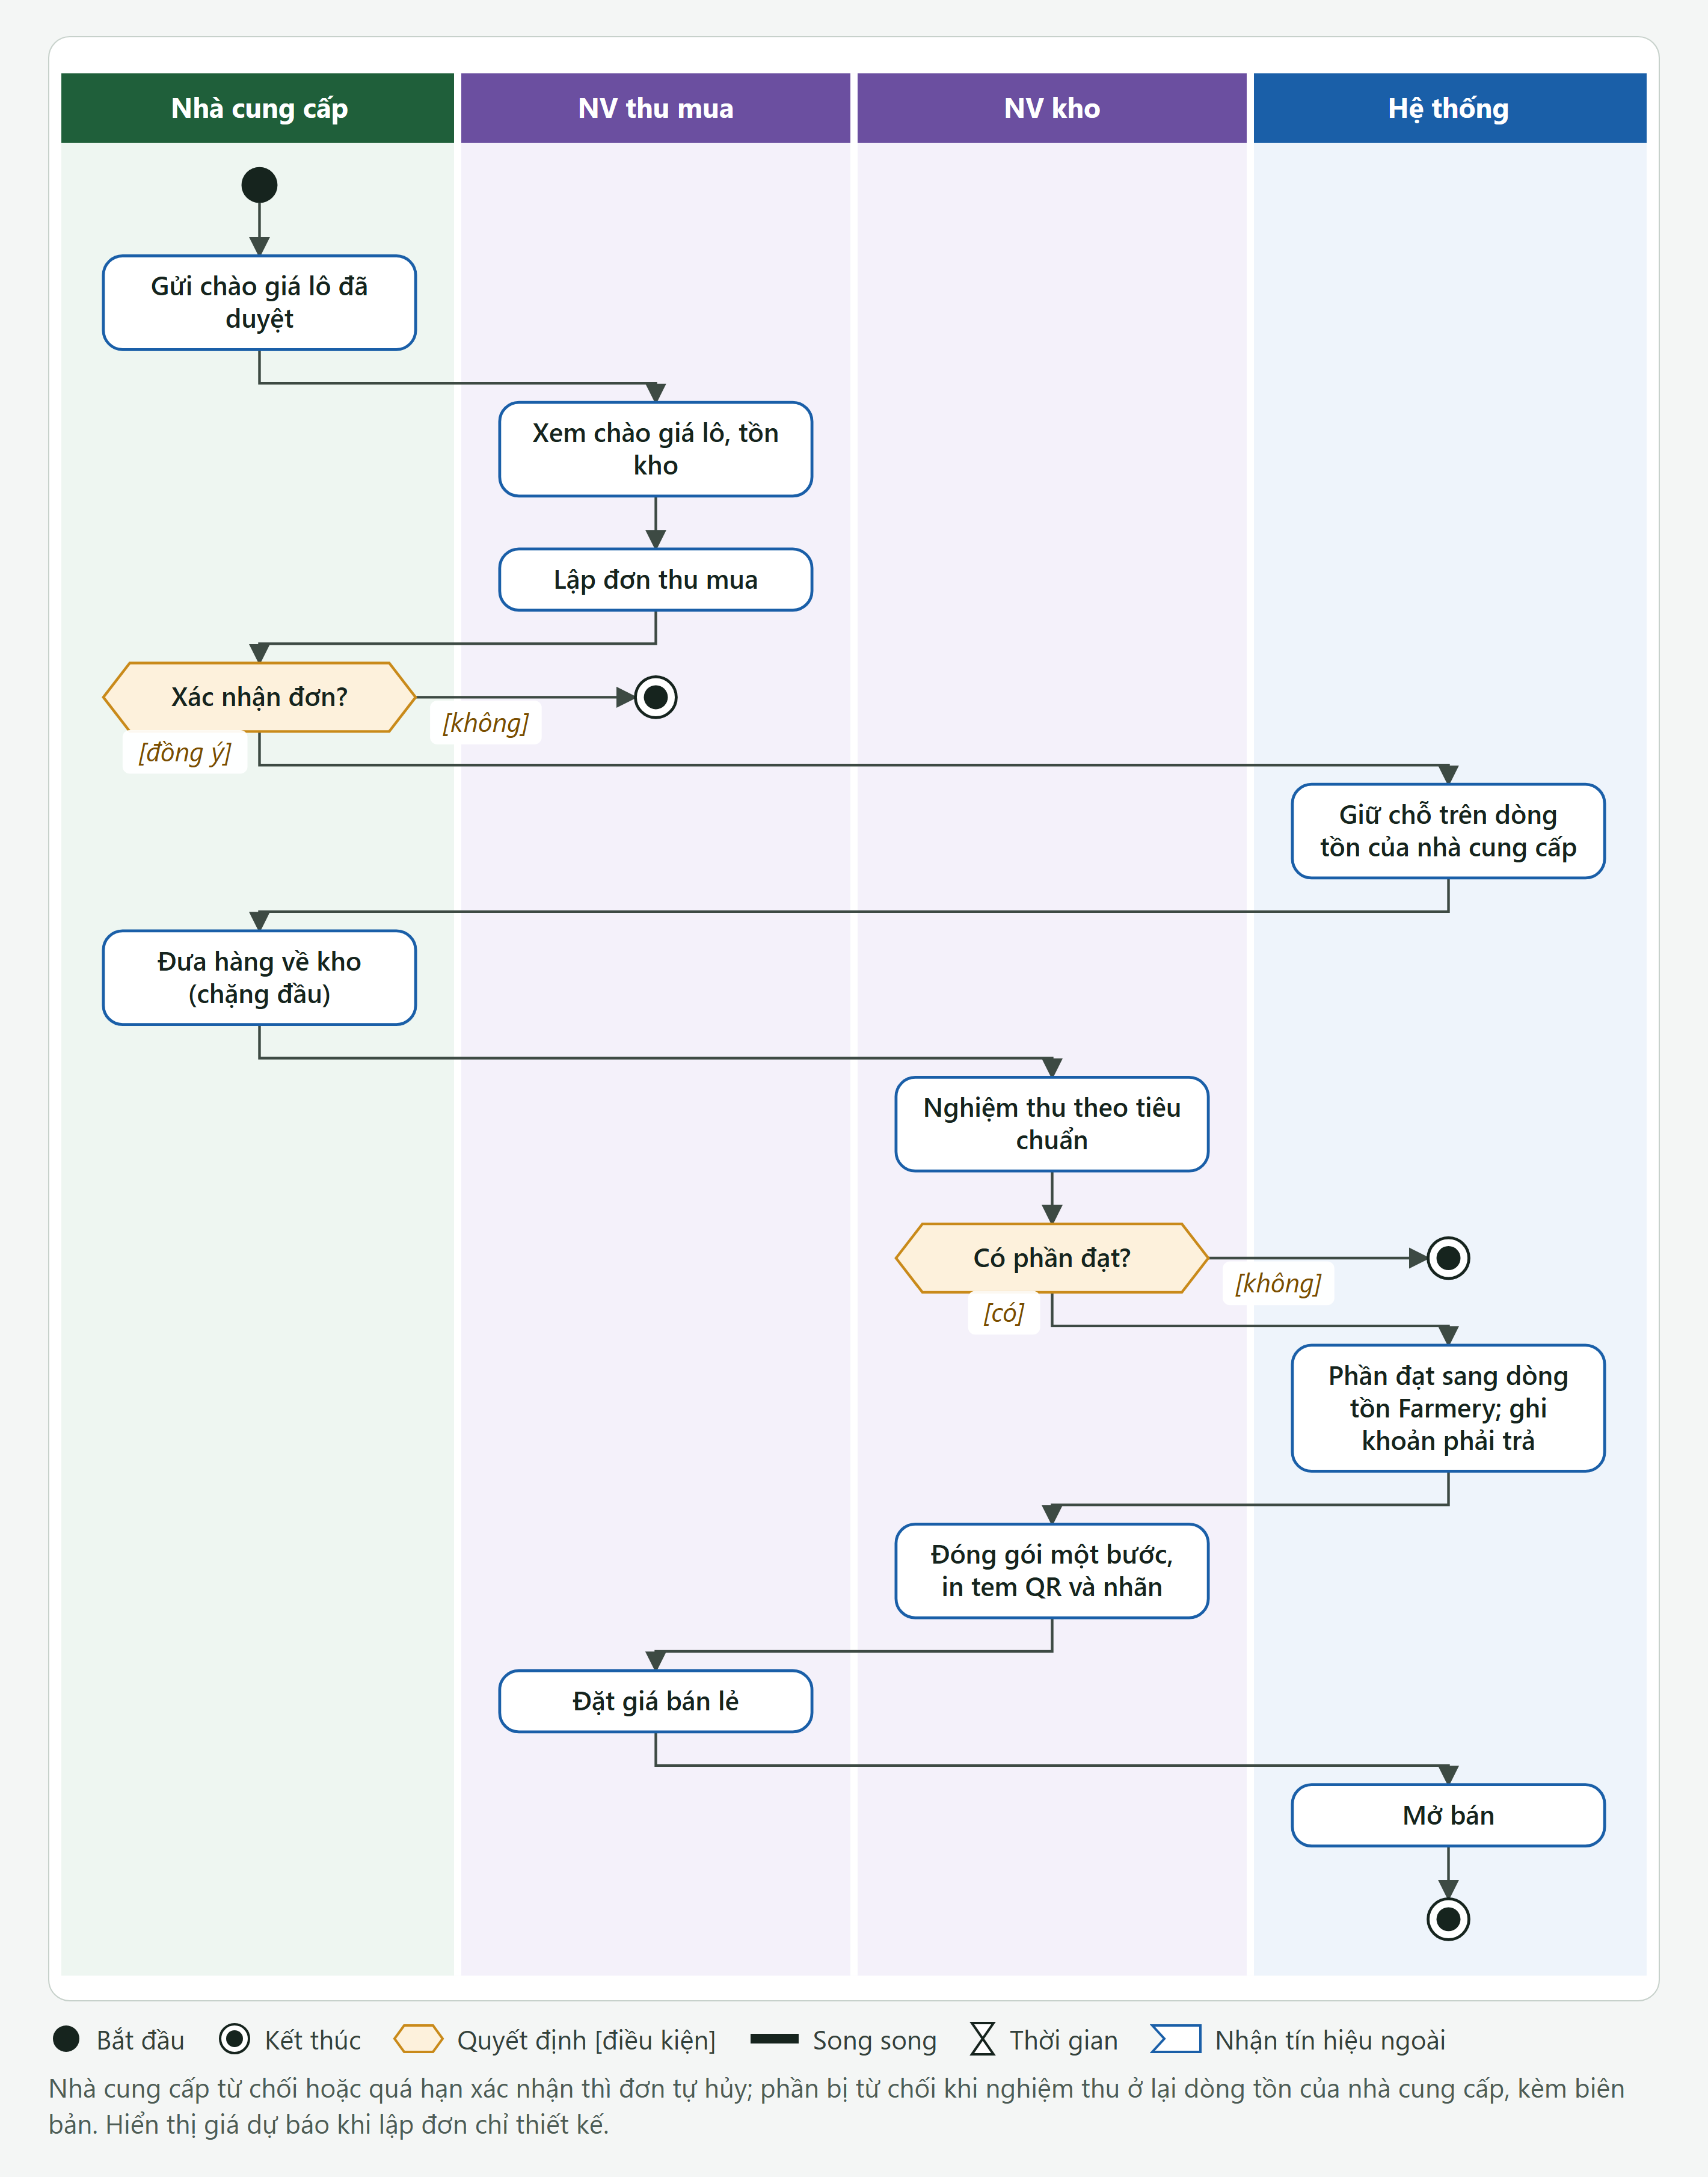
\includegraphics[width=\textwidth]{image/comparison/act-thu-mua.png}
\end{adjustbox}
\caption{Sơ đồ hoạt động: thu mua, nghiệm thu, đóng gói và đặt giá bán lẻ}
\label{fig:act-thu-mua}
\end{figure}

\begin{figure}[H]
\centering
\begin{adjustbox}{max totalsize={\textwidth}{0.62\textheight},center}
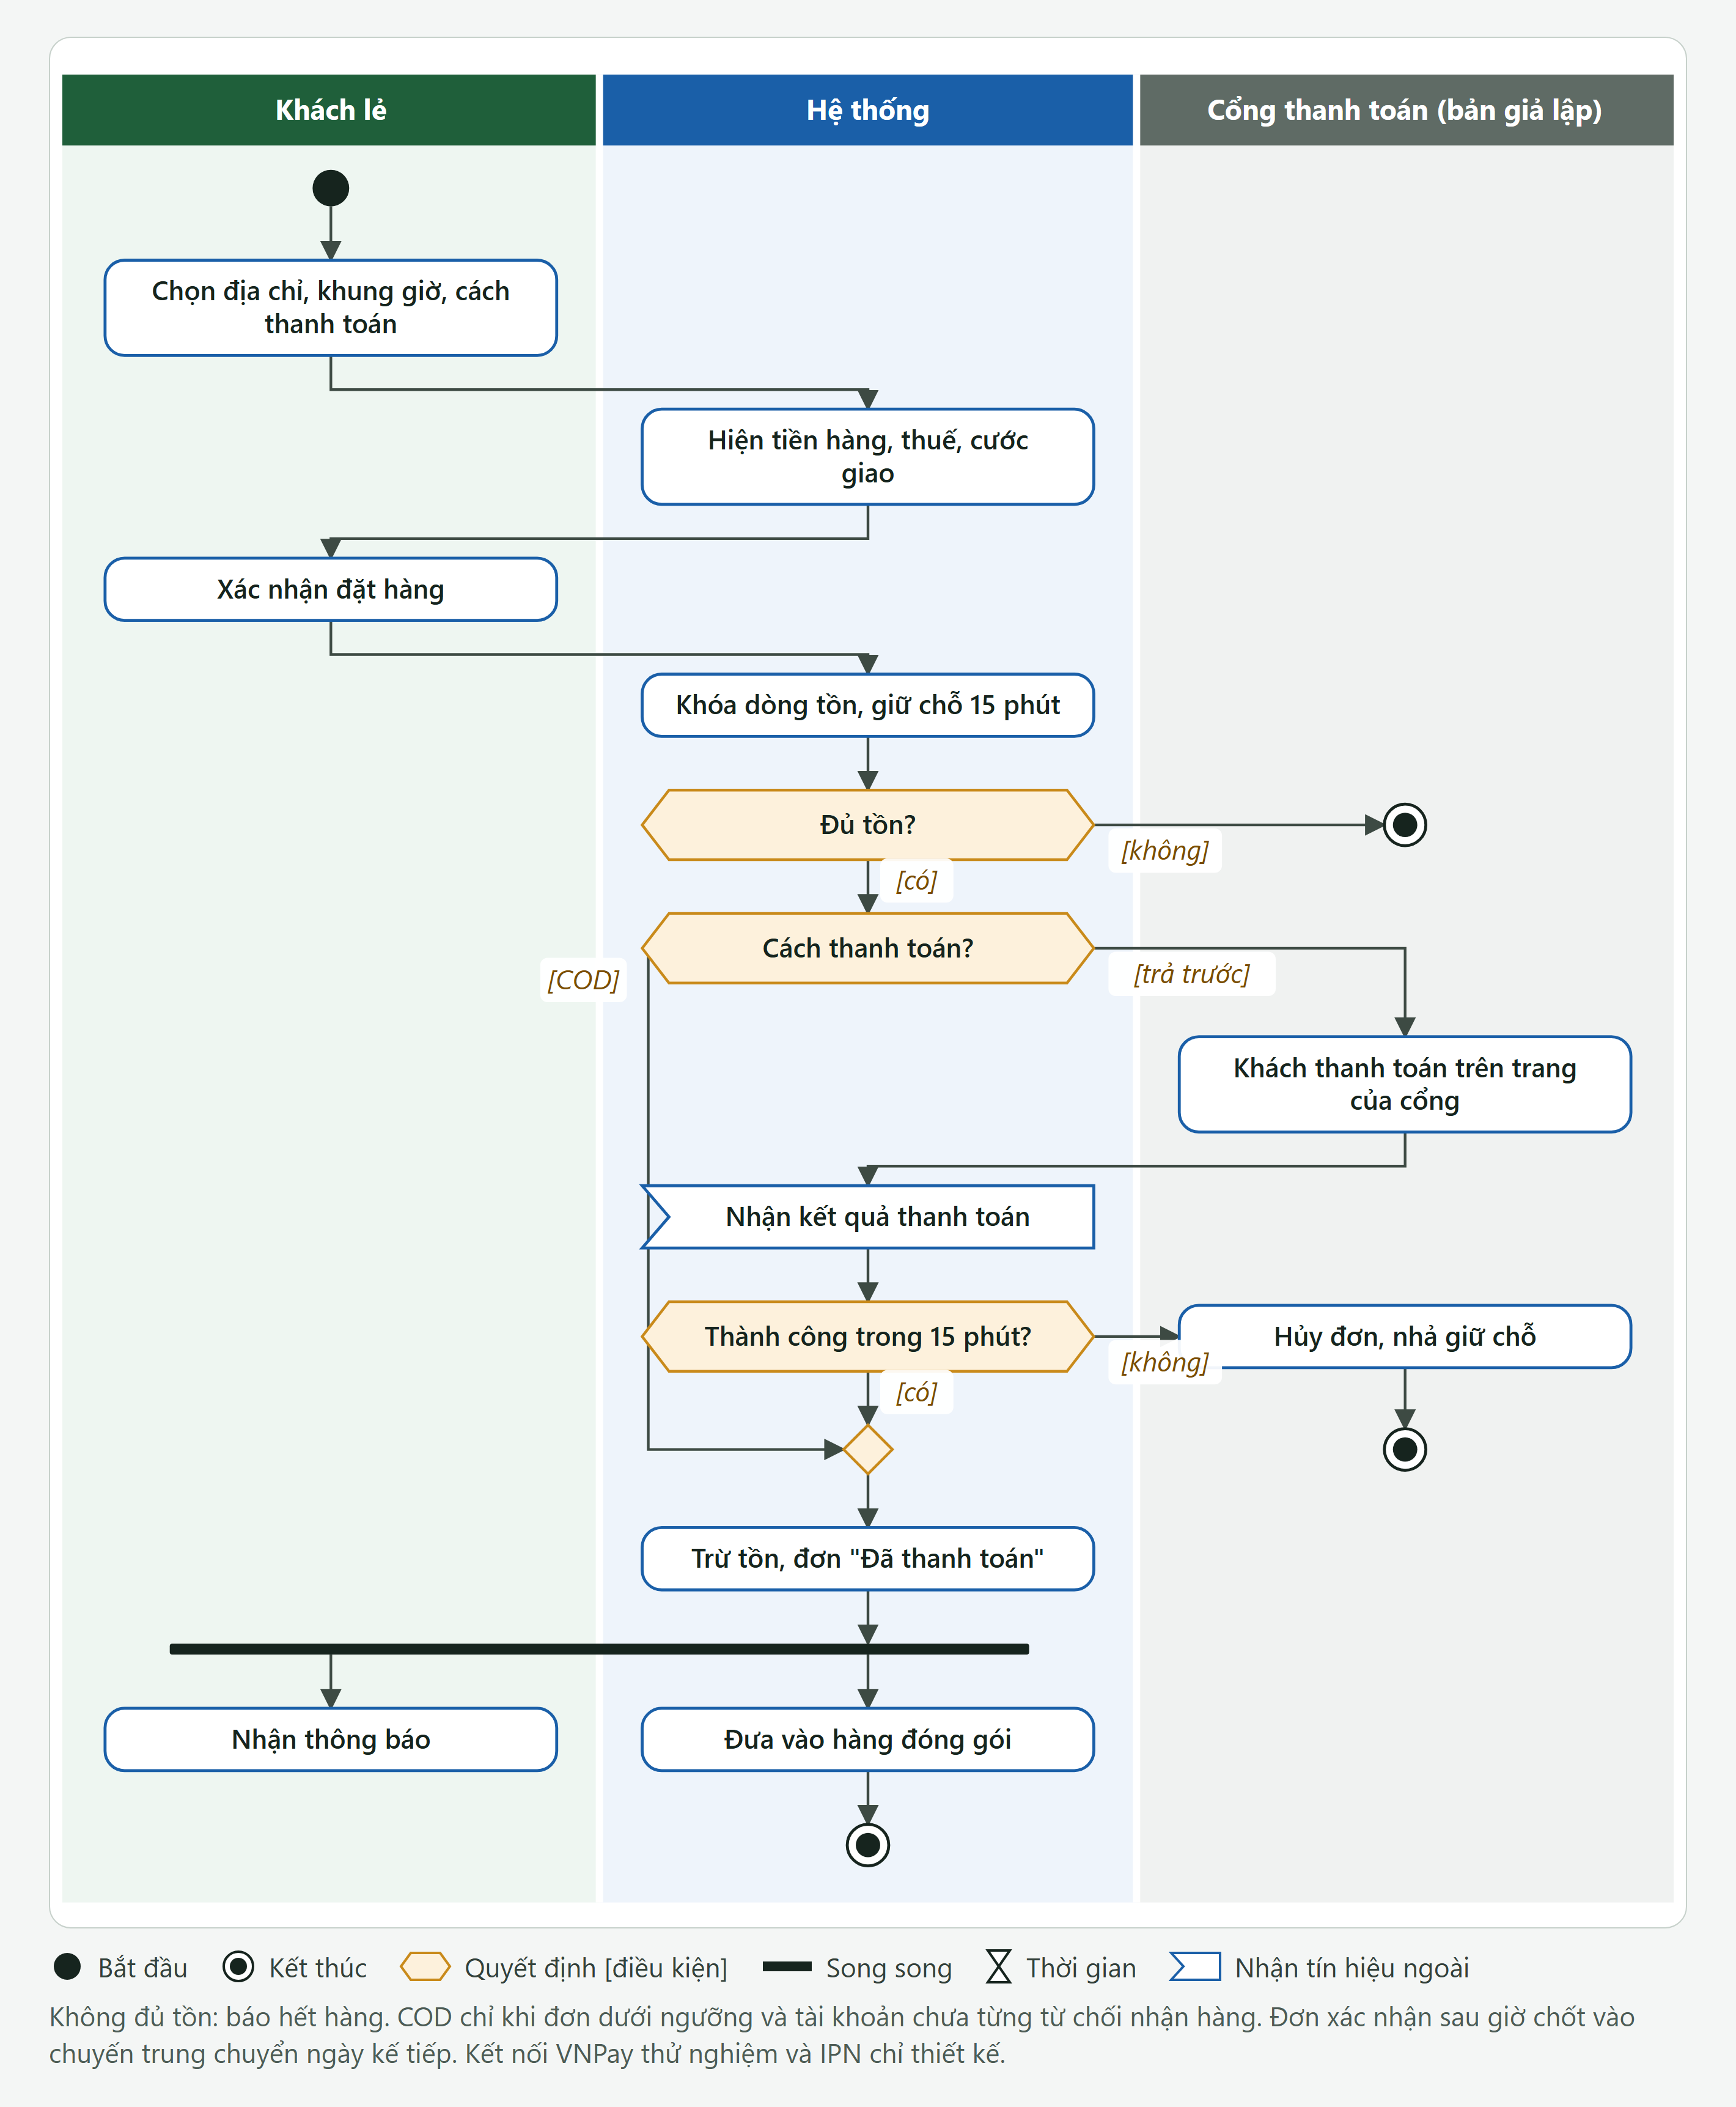
\includegraphics[width=\textwidth]{image/comparison/act-dat-hang.png}
\end{adjustbox}
\caption{Sơ đồ hoạt động: đặt hàng, giữ chỗ tồn kho và thanh toán đơn lẻ}
\label{fig:act-dat-hang}
\end{figure}

\subsection{Mô hình hóa tương tác}
\label{sec:sddchitiet}

Các tác nhân khớp với vai trò RBAC ở mục~\ref{sec:doituongnguoidung}: khách vãng lai (tìm kiếm, quét QR, xem sản phẩm, đăng ký), khách lẻ (\texttt{buyer\_retail}, luồng 1P), khách sỉ (\texttt{buyer\_wholesale}, luồng 3P), nhà cung cấp (\texttt{seller}), sáu vai trò nội bộ và ba hệ thống bên ngoài (cổng thanh toán, hóa đơn điện tử đều giả lập; đơn vị vận chuyển \emph{chỉ thiết kế}). \emph{Khách vãng lai} và \emph{Nhân sự nội bộ} là hai tác nhân trừu tượng gom việc chung để sơ đồ gọn hơn; sáu vai trò nội bộ là các tập quyền độc lập, không kế thừa nhau (NFR3.1). Dịch vụ AI không phải tác nhân mà là thành phần bên trong hệ thống. Một use case phải do tác nhân bên ngoài khởi xướng để đạt mục tiêu của chính tác nhân đó; việc hệ thống tự làm (sinh QR khi lô được duyệt, sinh hợp đồng khi báo giá được chốt) là bước hoặc hậu điều kiện của use case.

Hình~\ref{fig:usecase-overview} là sơ đồ tổng quan, nhóm theo năm gói ứng với năm khối mô-đun (Bảng~\ref{tab:module-io}): cột trái là use case của người dùng bên ngoài, cột phải của nhân sự nội bộ; use case của trục bán lẻ viền đậm, use case chỉ thiết kế vẽ xám nét đứt; mũi tên từ use case tới hệ thống bên ngoài mà nó gọi.

\begin{figure}[H]
\centering
\begin{adjustbox}{max totalsize={\textwidth}{0.82\textheight},center}
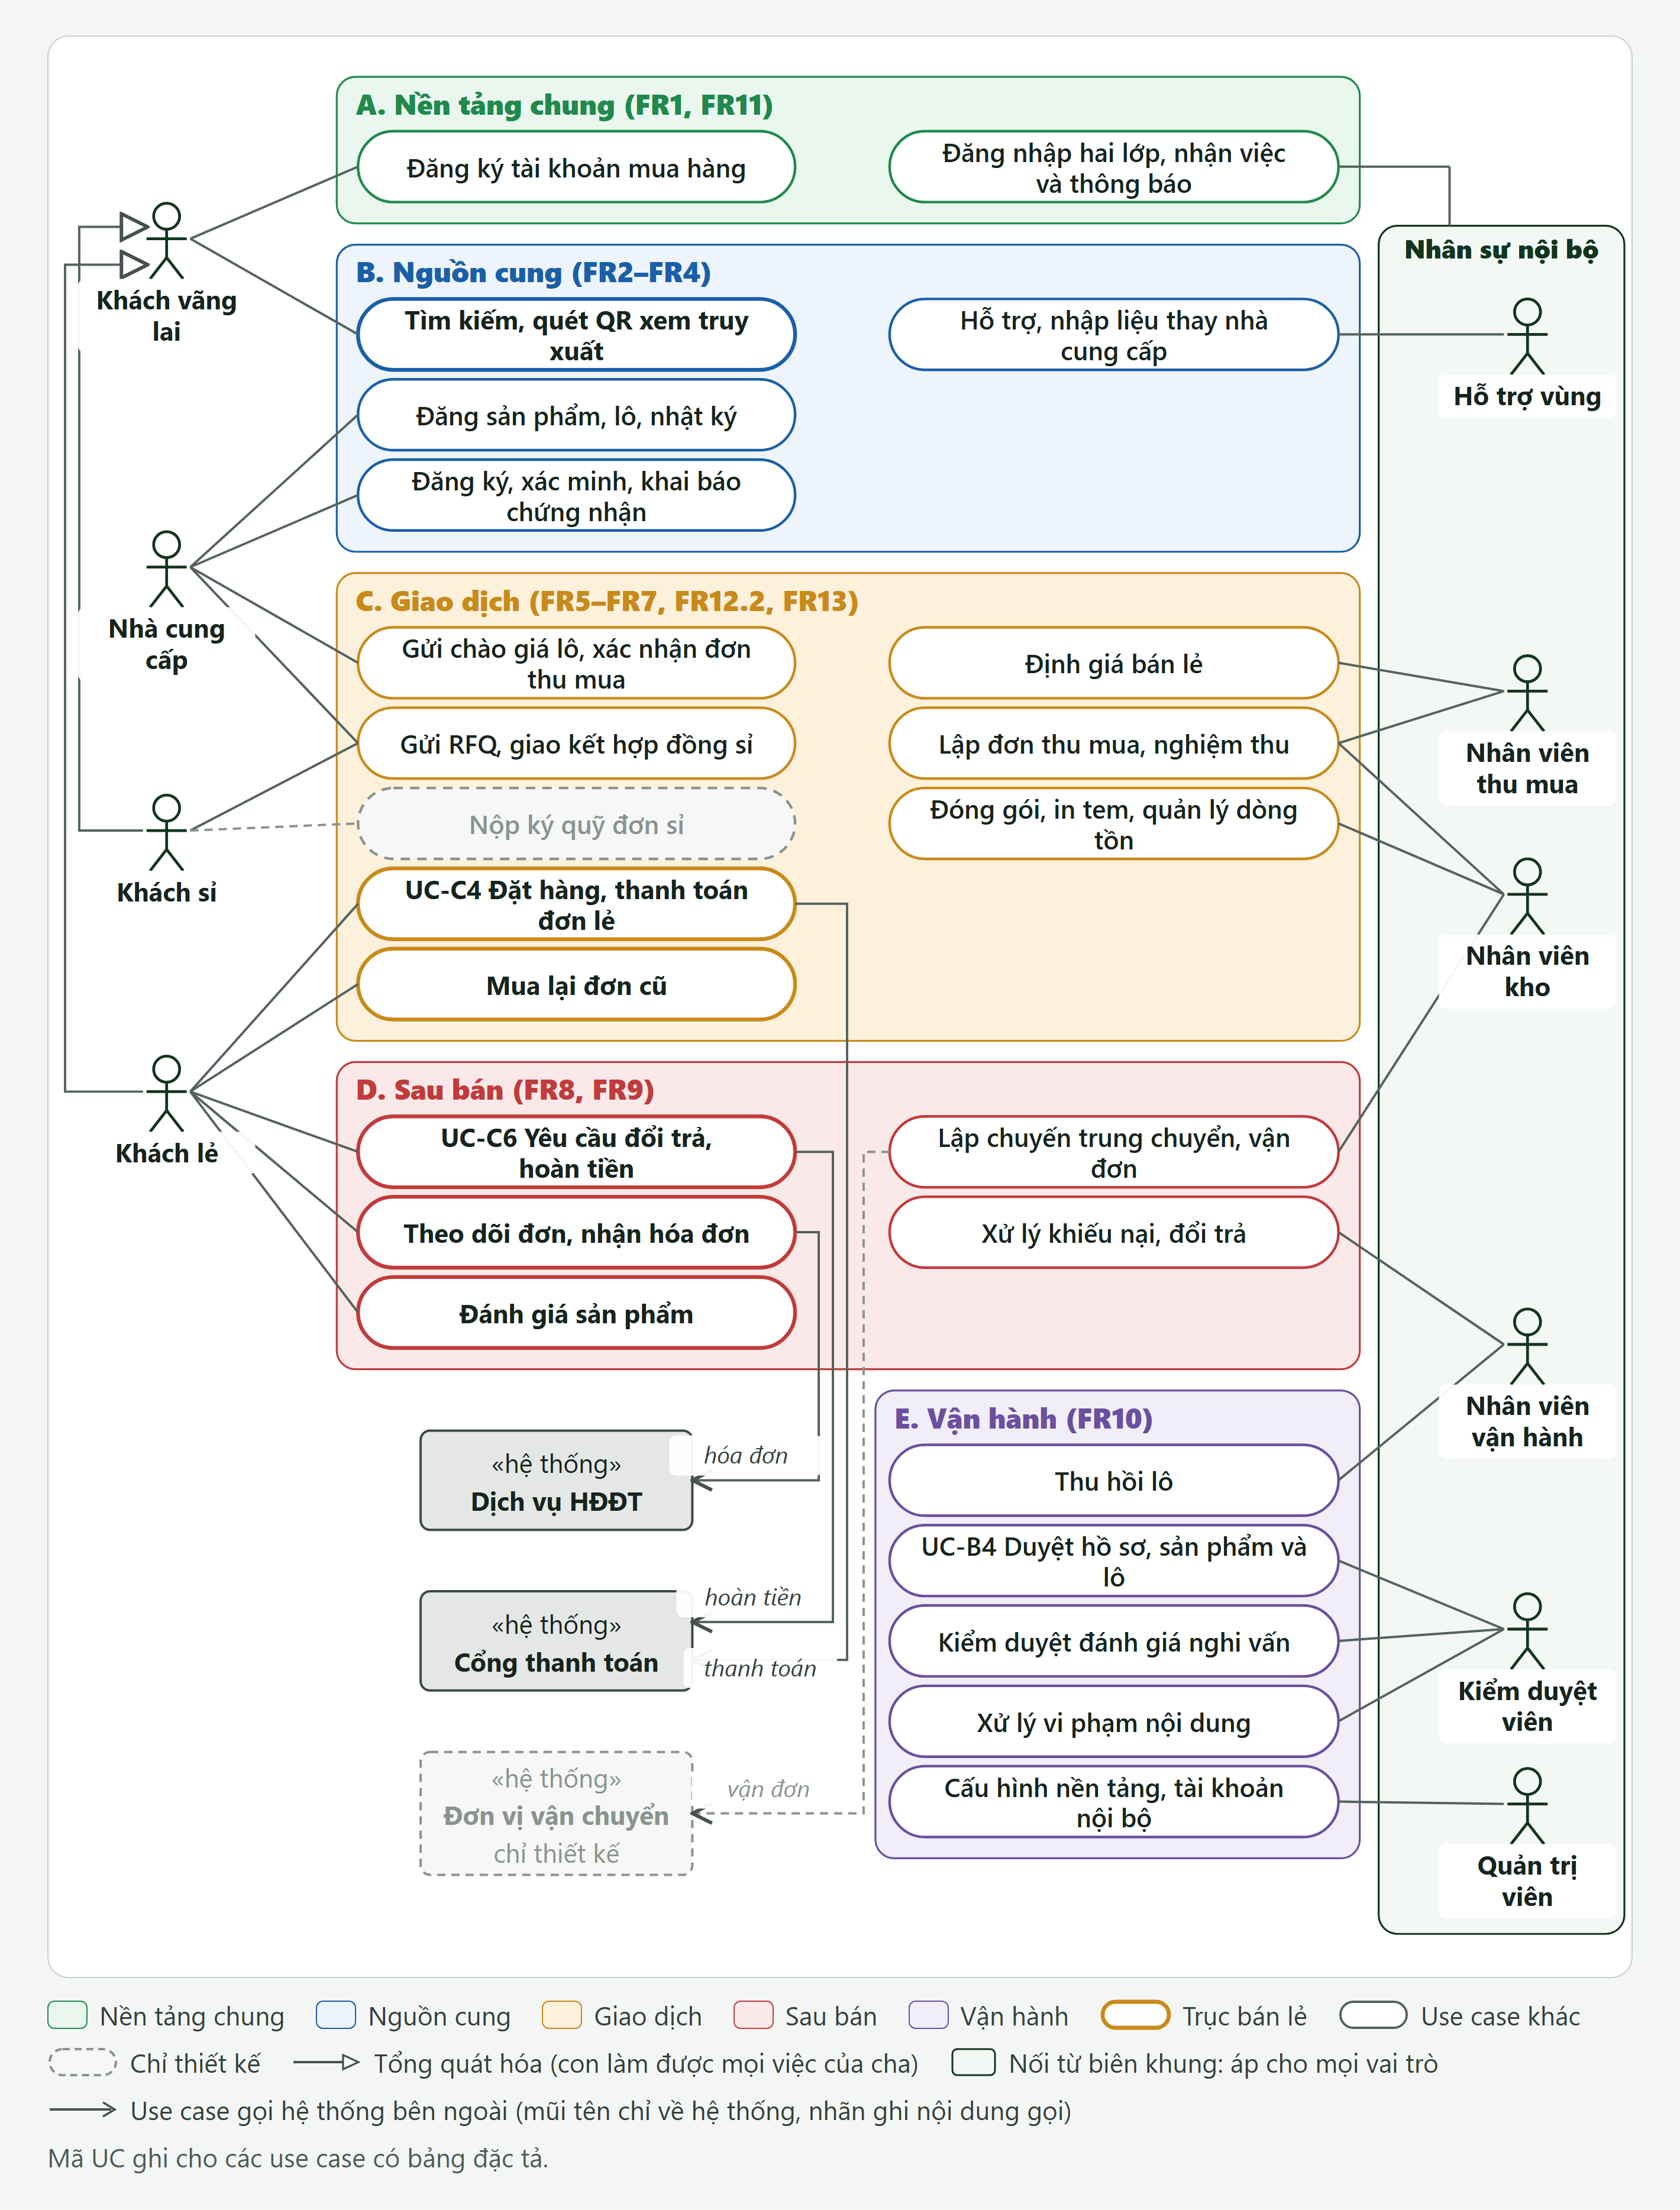
\includegraphics{image/comparison/usecase-overview.png}
\end{adjustbox}
\caption{Sơ đồ Use Case tổng quan hệ thống Farmery}
\label{fig:usecase-overview}
\end{figure}

Ba use case được đặc tả, chọn để đủ các loại luồng: UC-B4 (Bảng~\ref{tab:uc-b4}; nhân sự duyệt, hệ thống tự sinh mã QR), UC-C4 (Bảng~\ref{tab:uc-c4}; trục bán lẻ có hệ thống bên ngoài), UC-C6 (Bảng~\ref{tab:uc-c6}; đổi trả, hai bên thao tác và rẽ nhánh theo quyết định).

\begingroup
\tblsetup
\begin{longtable}{L{3.00cm} L{12.25cm}}
\caption{Đặc tả use case UC-B4 --- Duyệt sản phẩm và lô hàng}
\label{tab:uc-b4} \\
\toprule
\rowcolor{tblheadbg}
\multicolumn{2}{l}{\textbf{UC-B4: Duyệt sản phẩm và lô hàng}} \\
\midrule
\endfirsthead
\bottomrule
\endfoot
\textbf{Actor chính} & Kiểm duyệt viên (\texttt{staff\_moderation}) \\
\textbf{Tiền điều kiện} & Sản phẩm và lô đã qua kiểm tra tự động sơ bộ (FR4.6); lô có tối thiểu một bản ghi nhật ký canh tác và ảnh sản phẩm thật \\
\textbf{Luồng chính} &
1. Kiểm duyệt viên mở hàng đợi duyệt, xem sản phẩm, nhật ký canh tác, chứng nhận liên quan.\newline
2. Đối chiếu mã số vùng trồng với cổng công bố của Bộ và ghi kết quả.\newline
3. Phê duyệt sản phẩm và lô.\newline
4. Hệ thống sinh mã định danh lô theo GS1 (GTIN kèm số lô) và mã QR dẫn tới trang truy xuất công khai.\newline
5. Hệ thống phát sự kiện \texttt{BatchApproved}: mô-đun tồn kho mở dòng tồn của nhà cung cấp cho lô; nhà cung cấp nhận thông báo. \\
\textbf{Ngoại lệ} & 3a. Không đạt: từ chối kèm lý do, nhà cung cấp nhận hướng dẫn bổ sung. 4a. Lô đã có QR (đính chính sau duyệt): không sinh mã mới, chỉ cập nhật trang truy xuất. \\
\textbf{Hậu điều kiện} & Sản phẩm hiển thị công khai; lô có QR quét được và dòng tồn sẵn sàng giao dịch. \\
\end{longtable}
\endgroup

\begingroup
\tblsetup
\begin{longtable}{L{3.00cm} L{12.25cm}}
\caption{Đặc tả use case UC-C4 --- Đặt hàng và thanh toán đơn bán lẻ}
\label{tab:uc-c4} \\
\toprule
\rowcolor{tblheadbg}
\multicolumn{2}{l}{\textbf{UC-C4: Đặt hàng và thanh toán đơn bán lẻ}} \\
\midrule
\endfirsthead
\bottomrule
\endfoot
\textbf{Actor} & Khách lẻ (chính); cổng thanh toán (phụ) \\
\textbf{Tiền điều kiện} & Khách đã đăng nhập; giỏ hàng có ít nhất một sản phẩm còn bán \\
\textbf{Luồng chính} &
1. Khách chọn địa chỉ, khung giờ, cách thanh toán; hệ thống hiển thị tiền hàng, thuế, cước (FR5.2, FR8.2).\newline
2. Khách xác nhận; hệ thống khóa dòng tồn của Farmery và giữ chỗ 15 phút, đơn ``Đã đặt''.\newline
3. Hệ thống tạo giao dịch, chuyển khách sang cổng thanh toán; cổng xử lý và gửi kết quả (bản hiện thực dùng cổng giả lập; kết nối VNPay và IPN \emph{chỉ thiết kế}).\newline
4. Hệ thống chuyển đơn ``Đã thanh toán'', đổi giữ chỗ thành trừ tồn, đưa đơn vào hàng đóng gói, thông báo khách. \\
\textbf{Ngoại lệ} & COD: chỉ khi đơn dưới ngưỡng và tài khoản chưa từng từ chối nhận hàng, bỏ qua bước 3, đơn xác nhận ngay. Không đủ tồn: báo khách bỏ sản phẩm hoặc giảm số lượng. Thanh toán thất bại hoặc quá 15 phút: hủy đơn, nhả giữ chỗ. Xác nhận sau giờ chốt: vào chuyến trung chuyển ngày kế tiếp. \\
\textbf{Hậu điều kiện} & Đơn ``Đã thanh toán'' (hoặc COD đã xác nhận) và tồn đã trừ; hoặc đơn bị hủy và tồn trở về như trước khi đặt. \\
\end{longtable}
\endgroup

\begingroup
\tblsetup
\begin{longtable}{L{3.00cm} L{12.25cm}}
\caption{Đặc tả use case UC-C6 --- Yêu cầu đổi trả, hoàn tiền đơn lẻ}
\label{tab:uc-c6} \\
\toprule
\rowcolor{tblheadbg}
\multicolumn{2}{l}{\textbf{UC-C6: Yêu cầu đổi trả, hoàn tiền đơn lẻ}} \\
\midrule
\endfirsthead
\bottomrule
\endfoot
\textbf{Actor} & Khách lẻ (chính); nhân viên vận hành ra quyết định; cổng thanh toán (hoàn tiền) \\
\textbf{Tiền điều kiện} & Đơn ``Đã giao'' và còn trong thời hạn khiếu nại của nhóm hàng (rau lá 24 giờ, củ quả 48 giờ, hàng khô 7 ngày) \\
\textbf{Luồng chính} &
1. Khách chọn đơn, sản phẩm, lý do, đính kèm ảnh hoặc video.\newline
2. Hệ thống kiểm tra thời hạn, tạo yêu cầu vào hàng đợi có hạn xử lý; khách nhận xác nhận trong 24 giờ.\newline
3. Nhân viên vận hành xem minh chứng, yêu cầu bổ sung ngay trên yêu cầu nếu cần.\newline
4. Trong 3 ngày làm việc, nhân viên quyết định hoàn tiền không cần trả hàng, đổi hàng hoặc từ chối kèm lý do; mỗi lần đổi trạng thái hệ thống email cho khách.\newline
5. Nếu hoàn tiền: hệ thống ra lệnh hoàn qua cổng và ghi bút toán hủy vào sổ nhập xuất; tiền về trong 7 ngày làm việc. \\
\textbf{Ngoại lệ} & Quá hạn hoặc hàng tươi trả vì đổi ý: không tạo yêu cầu, nêu chính sách. Giá trị vượt ngưỡng hoàn tiền không cần trả hàng: yêu cầu gửi trả, hàng về kho được ghi sổ trước khi hoàn. Lỗi của đơn vị vận chuyển: Farmery xử lý với khách trước, đòi lại sau. Quá hạn xử lý: tự nâng ưu tiên (FR10.3). \\
\textbf{Hậu điều kiện} & Yêu cầu đóng với quyết định có lý do; nếu hoàn tiền thì giao dịch hoàn đã ghi ở cả cổng thanh toán và sổ nhập xuất. \\
\end{longtable}
\endgroup

\section{Giải pháp công nghệ}
\label{sec:giaiphapcongnghe}

Mỗi hạng mục được quyết định bằng cách nêu phương án ứng viên, đối chiếu theo năm tiêu chí chung rồi chọn: đáp ứng yêu cầu phi chức năng (mục~\ref{sec:yeucauphichucnang}), phù hợp đặc thù nông sản (dữ liệu theo lô, nhiều ảnh, tìm theo vùng và mùa vụ), độ trưởng thành và hệ sinh thái, chi phí (ưu tiên mã nguồn mở hoặc gói miễn phí), và chi phí học của nhóm. Nguyên tắc xuyên suốt là \textbf{giảm tối đa số thành phần hạ tầng phải vận hành}, vì mỗi thành phần thêm vào kéo theo chi phí cài đặt, giám sát và đồng bộ dữ liệu. Bảng~\ref{tab:congnghe} nêu kết luận; đối sánh các hướng tiếp cận AI ở Phụ lục~F.

\begingroup
\tblsetup\tblzebra
\begin{longtable}{L{2.90cm} L{3.40cm} L{8.95cm}}
\caption{Lựa chọn công nghệ và lý do chính}
\label{tab:congnghe} \\
\toprule
\rowcolor{tblheadbg}
\textbf{Hạng mục} & \textbf{Chọn} & \textbf{Lý do chính (phương án đã loại)} \\
\midrule
\endfirsthead
\toprule
\rowcolor{tblheadbg}
\textbf{Hạng mục} & \textbf{Chọn} & \textbf{Lý do chính (phương án đã loại)} \\
\midrule
\endhead
\bottomrule
\endfoot
Ứng dụng mua hàng & Next.js, PWA & Trang truy xuất và trang sản phẩm mở công khai qua QR, cần SSR và lập chỉ mục; service worker cho hàng đợi ngoại tuyến (NFR7.3). Loại Vue/Nuxt, Angular \\
Ứng dụng nội bộ & React, Vite, Refine & Chủ yếu danh sách, biểu mẫu, hàng đợi theo vai trò, không cần SSR; tách khỏi Next.js để mã màn hình quyền cao không nằm trong gói tải xuống của khách. Loại React-Admin \\
Kho mã & Monorepo pnpm, Turborepo & Chia sẻ kiểu dữ liệu sinh từ API, chỉ dựng lại phần bị ảnh hưởng. Loại tách nhiều kho (đồng bộ kiểu bằng tay), Nx (cấu hình nặng) \\
Framework máy chủ & NestJS (Node.js, TypeScript) & Chung ngôn ngữ với giao diện; mô-đun và guard phù hợp phân quyền nhiều vai trò (NFR3.6). Loại Spring Boot, Django/FastAPI, Laravel \\
Truy cập dữ liệu & Prisma & Lược đồ khai báo một nơi, sinh kiểu và migration; riêng giữ chỗ và trừ tồn viết SQL thô \texttt{SELECT \ldots{} FOR UPDATE} trong giao dịch, gom ở một lớp. Loại TypeORM, Drizzle \\
Cơ sở dữ liệu & PostgreSQL (pgvector) & Một mình đáp ứng ba nhu cầu: giao dịch có khóa dòng để chống bán vượt (NFR4.1), JSON có chỉ mục cho nhật ký canh tác, và vector cho tìm kiếm ngữ nghĩa (FR12.3) không cần cơ sở dữ liệu vector riêng. Loại MySQL, MongoDB \\
Tìm kiếm và lọc & Full-text của PostgreSQL & Đủ cho 100 người dùng đồng thời (NFR1.1) và các bộ lọc FR4.5; search engine riêng phát sinh bài toán đồng bộ. Chuyển khi truy vấn vượt ngưỡng NFR1.1 \\
Lưu trữ tệp & MinIO (S3) & Không phình cơ sở dữ liệu, không cản nhân bản ngang (NFR2.2) \\
Sự kiện và cache & Bus sự kiện trong tiến trình; Redis \emph{(chỉ thiết kế)} & Bản hiện thực phát và nhận sự kiện ngay trong máy chủ (bên nhận chỉ xử lý một lần); Redis làm hàng đợi bền và cache đọc nhiều khi cần chạy nhiều bản sao máy chủ. Không cần message broker riêng \\
Thanh toán & VNPay (thử nghiệm) & Gom nhiều phương thức sau một lần tích hợp, có môi trường thử nghiệm; PayOS cho VietQR. Kết nối thật \emph{chỉ thiết kế}, bản hiện thực dùng giả lập \\
Vận chuyển chặng cuối & GHN (thử nghiệm) & Có API vận đơn, webhook, môi trường thử nghiệm; chặng giữa do nhân viên kho cập nhật. \emph{Chỉ thiết kế} \\
Hóa đơn điện tử & Lớp tích hợp, bản giả lập & Cùng giao diện với nhà cung cấp thật (VNPT, Viettel, MISA); kết nối thật cần hợp đồng và chứng thư số \\
Thông báo & Thông báo web, email SMTP & Web Push (chuẩn W3C, khóa VAPID) và SMS \emph{chỉ thiết kế}; trang đơn tự hỏi lại trạng thái mỗi 5 giây \\
\end{longtable}
\endgroup

Ba mô-đun AI tách thành một dịch vụ riêng bằng Python và FastAPI vì toàn bộ thư viện học máy cần dùng thuộc hệ sinh thái Python; mô hình bám theo ngưỡng ở Bảng~\ref{tab:nguongAI}.
\begin{itemize}
    \item \textbf{Tìm kiếm ngữ nghĩa:} tìm kiếm lai giữa full-text PostgreSQL (\texttt{unaccent} cho gõ không dấu, \texttt{pg\_trgm} chịu gõ sai) và tìm theo vector BGE-M3 \parencite{chen2024bgem3}, hợp nhất bằng reciprocal rank fusion. Không tốn phí gọi API, giữ điểm mạnh của từ khóa với tên riêng và vùng trồng, có sẵn đường cơ sở để so sánh (FR4.5). Loại tìm theo vector thuần túy, mô hình ngôn ngữ lớn chuyển câu hỏi thành bộ lọc, và tìm kiếm hội thoại (thực chất là trợ lý ảo đã bỏ khỏi phạm vi).
    \item \textbf{Gợi ý sản phẩm:} mô hình hybrid hai giai đoạn. Phần hiện thực là ``sản phẩm tương tự'' tính từ vector sản phẩm, đo bằng Precision@5; phần theo hành vi chỉ thiết kế. Hybrid cho phép dựa vào đặc trưng nông sản (mùa vụ, vùng trồng, chứng nhận) khi chưa có lịch sử tương tác (NC4).
    \item \textbf{Dự báo giá:} chuỗi thời gian có mùa vụ (ARIMA, SARIMA, Prophet), đối chứng gradient boosting. Học sâu bị loại vì cần nhiều dữ liệu hơn mức thu thập được; với chuỗi ngắn nhưng mùa vụ rõ, mô hình thống kê thường tốt hơn và dễ giải thích --- chọn mô hình đơn giản nhưng kiểm chứng được.
    \item \textbf{Giám sát bất thường} dùng luật ngưỡng do quản trị viên cấu hình (lý do ở Chương~\ref{chap:coso}).
\end{itemize}

\section{Thiết kế}
\label{sec:thietke}

\subsection{Thiết kế kiến trúc hệ thống}
\label{sec:kientruc}

Kiến trúc là hệ quả của các lựa chọn công nghệ trên, trình bày theo mô hình C4~\cite{brown_c4model}: mức 1 là ngữ cảnh (Hình~\ref{fig:c4-ngucanh}, mục~\ref{sec:luongvanhanh}); mức 2 là bảy container (Hình~\ref{fig:c4-container}, Bảng~\ref{tab:container-io}); mức 3 là 13 mô-đun của máy chủ nghiệp vụ (Hình~\ref{fig:c4-module}). Mức 4 (mã nguồn) không vẽ tay mà nên sinh tự động khi cần. Quy ước mũi tên chung: hai chiều khi bên được gọi trả dữ liệu nghiệp vụ về (nhãn ghi phần gửi trước dấu chấm phẩy, phần nhận sau); một chiều khi chỉ gửi đi; mũi tên chạm biên một khung áp cho mọi phần tử trong khung.

\begin{figure}[H]
\centering
\begin{adjustbox}{max totalsize={\textwidth}{0.62\textheight},center}
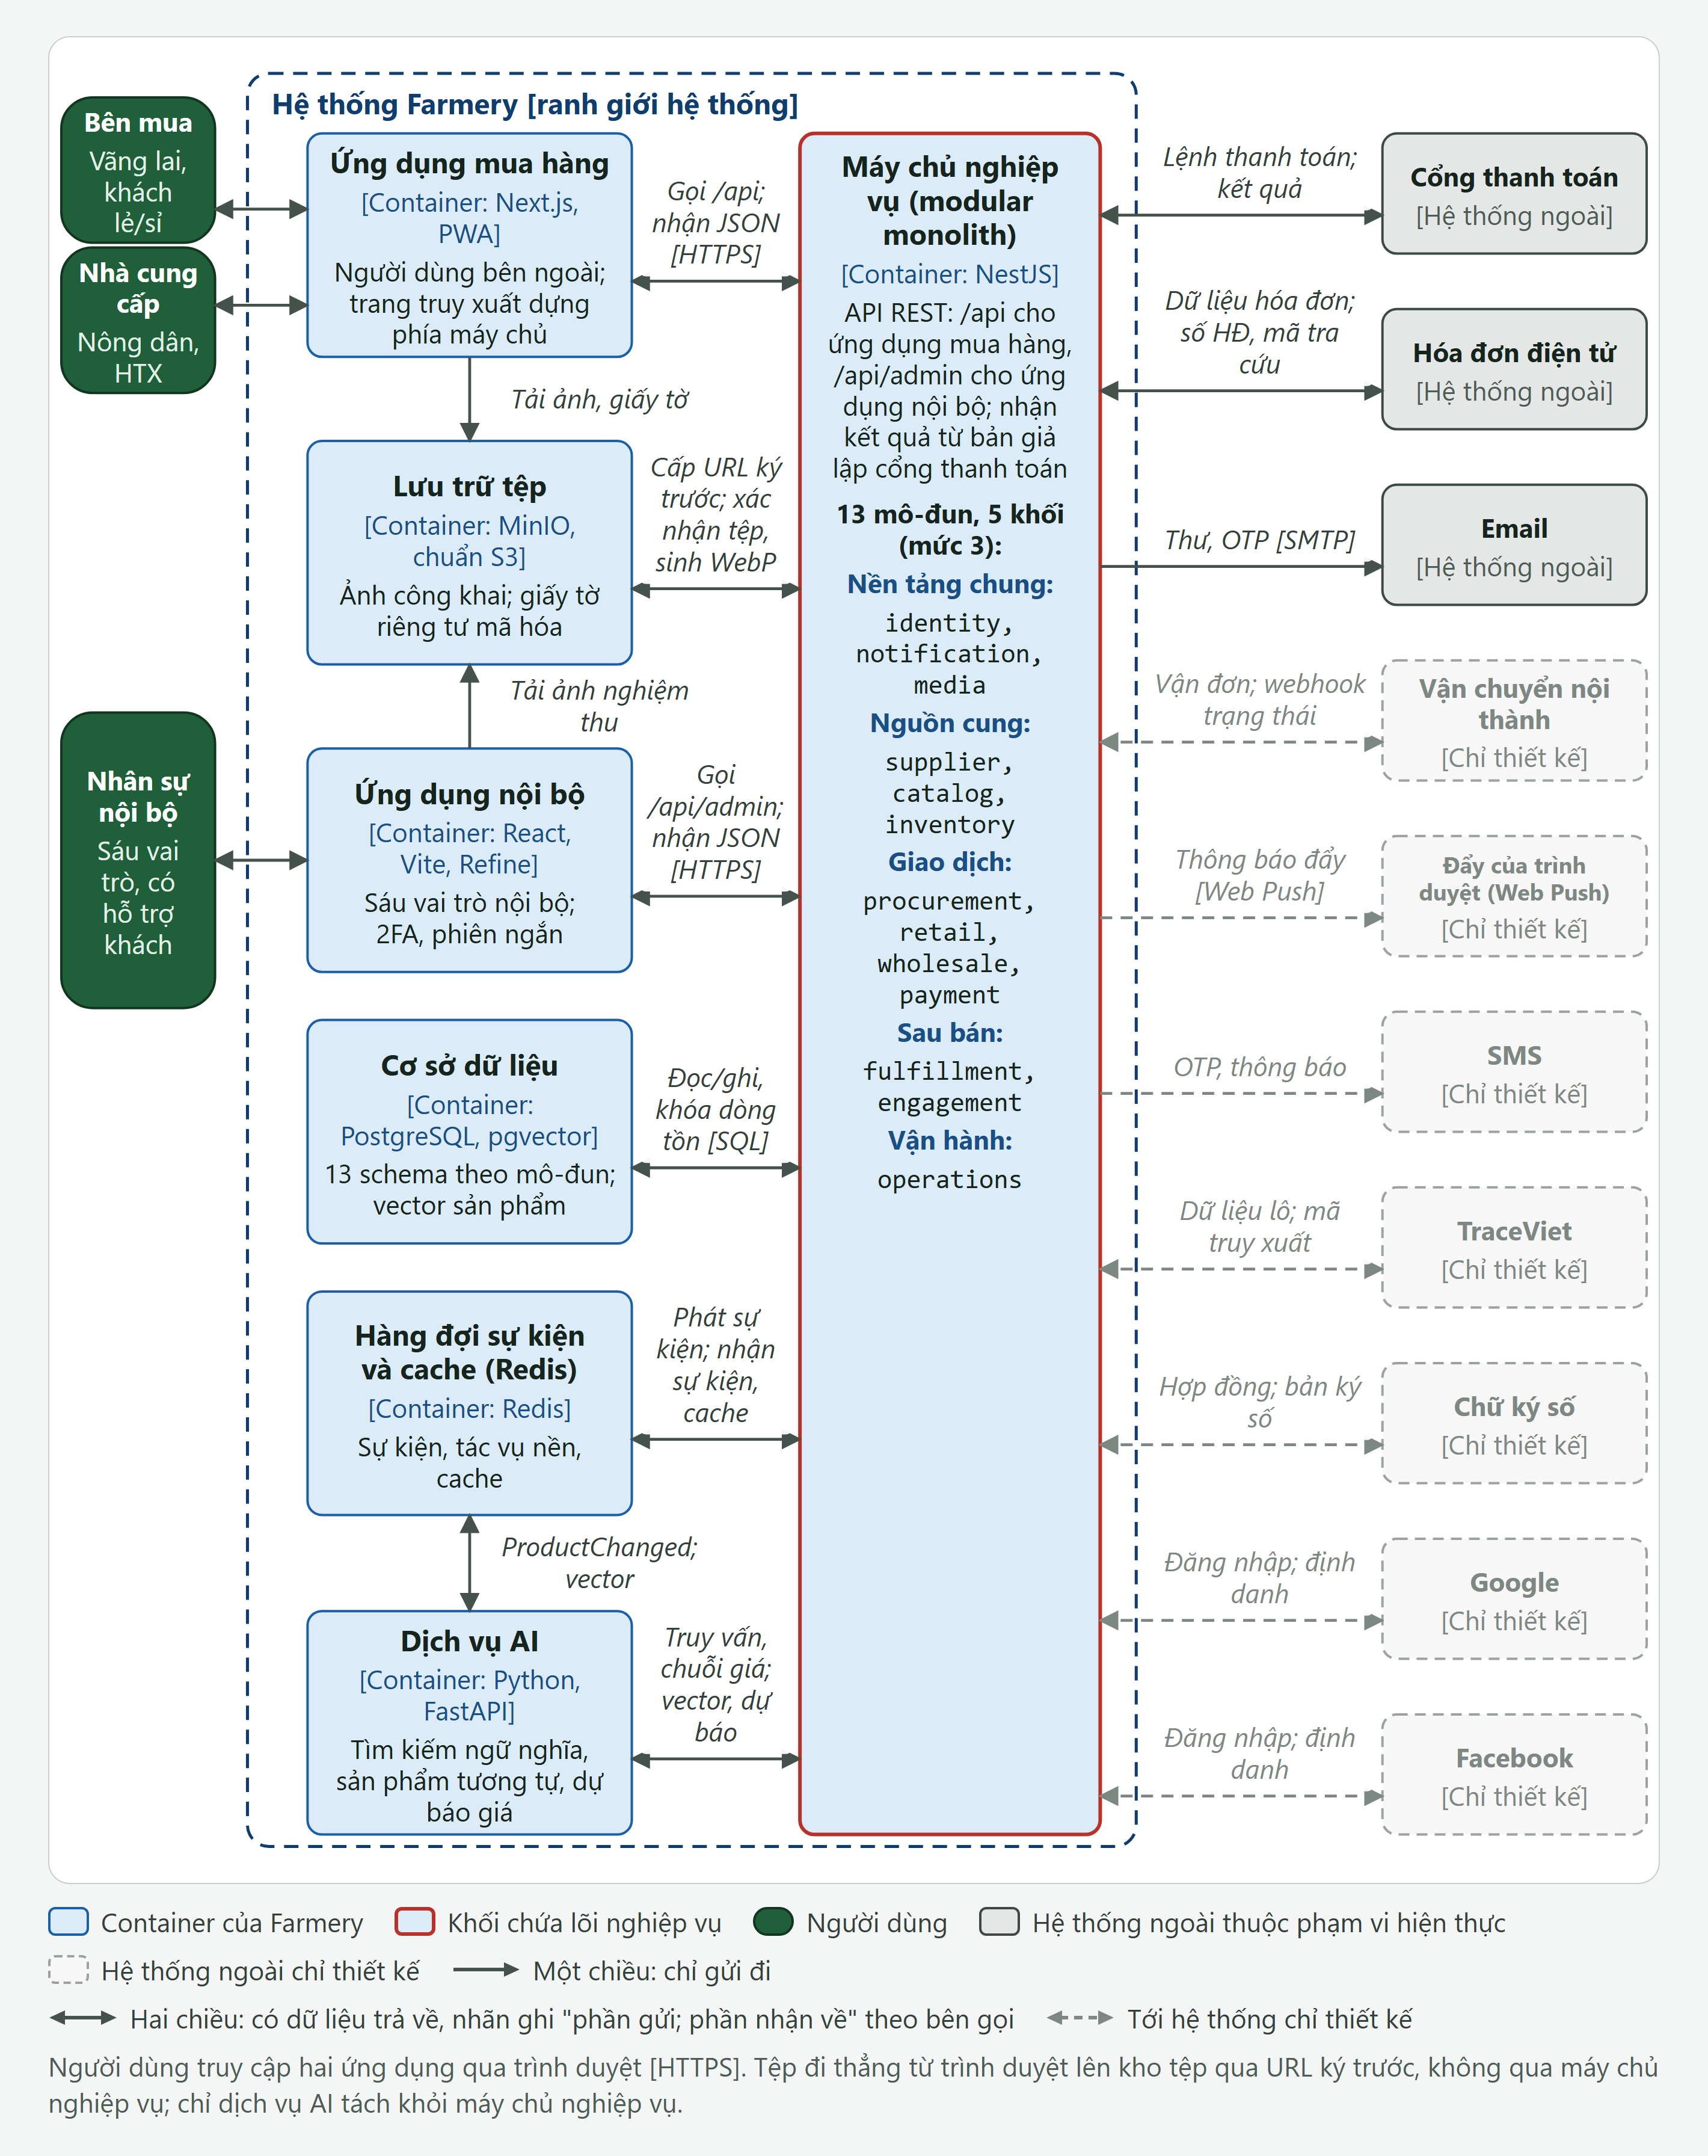
\includegraphics[width=\textwidth]{image/comparison/c4-container.png}
\end{adjustbox}
\caption{Kiến trúc tổng thể của Farmery: các container (C4 mức 2)}
\label{fig:c4-container}
\end{figure}

Hai điểm đáng chú ý ở Bảng~\ref{tab:container-io}: tệp đi thẳng từ trình duyệt lên kho tệp qua đường dẫn ký trước nên máy chủ không trung chuyển ảnh lớn; dịch vụ AI không đọc cơ sở dữ liệu mà nhận dữ liệu qua sự kiện hoặc lời gọi (\texttt{ProductChanged}) và trả vector qua sự kiện \texttt{ProductEmbedded} để mô-đun sản phẩm tự lưu, nên nếu dịch vụ AI ngừng, tìm kiếm lùi về từ khóa và trang chủ lùi về sản phẩm bán chạy, giao dịch không gián đoạn. Sự kiện đi qua một cổng phát sự kiện nên mô-đun phát không phải gọi và chờ từng mô-đun nhận; bản hiện thực chạy cổng này trong tiến trình máy chủ, còn Redis (hàng đợi bền và cache) chỉ thiết kế và thay vào mà không phải sửa nơi phát. Giao dịch ghi như khóa dòng tồn chạy thẳng trên cơ sở dữ liệu.

\begingroup
\tblsetup\tblzebra
\begin{longtable}{L{2.60cm} L{2.40cm} L{5.00cm} L{4.85cm}}
\caption{Dữ liệu vào, ra của từng container}
\label{tab:container-io} \\
\toprule
\rowcolor{tblheadbg}
\textbf{Container} & \textbf{Công nghệ} & \textbf{Nhận vào} & \textbf{Trả ra, ghi ra} \\
\midrule
\endfirsthead
\toprule
\rowcolor{tblheadbg}
\textbf{Container} & \textbf{Công nghệ} & \textbf{Nhận vào} & \textbf{Trả ra, ghi ra} \\
\midrule
\endhead
\bottomrule
\endfoot
Ứng dụng mua hàng & Next.js, PWA & Thao tác của khách và nhà cung cấp & Lời gọi \texttt{/api}; tệp tải thẳng lên kho tệp; trang truy xuất dựng sẵn phía máy chủ \\
Ứng dụng nội bộ & React, Vite, Refine & Thao tác sáu vai trò sau đăng nhập hai lớp & Lời gọi \texttt{/api/admin}; ảnh nghiệm thu tải thẳng lên kho tệp \\
Máy chủ nghiệp vụ & NestJS, 13 mô-đun & Yêu cầu REST; kết quả của dịch vụ AI; webhook bên ngoài \emph{(chỉ thiết kế)} & Phản hồi JSON; sự kiện qua bus sự kiện (Redis \emph{chỉ thiết kế}); lời gọi hệ thống ngoài \\
Cơ sở dữ liệu & PostgreSQL, pgvector & Đọc, ghi của từng mô-đun trên schema riêng & Dữ liệu nghiệp vụ; kết quả tìm kiếm toàn văn và vector \\
Lưu trữ tệp & MinIO (S3) & Tệp tải lên qua đường dẫn ký trước & Ảnh công khai WebP nhiều cỡ; tệp riêng tư qua đường dẫn hạn ngắn \\
Sự kiện và cache & Bus trong tiến trình; Redis \emph{(chỉ thiết kế)} & Sự kiện, tác vụ nền, dữ liệu đọc nhiều & Sự kiện cho mô-đun và dịch vụ AI đã đăng ký \\
Dịch vụ AI & Python, FastAPI & \texttt{ProductChanged}; câu truy vấn; chuỗi giá theo tháng (offline) & Vector sản phẩm, vector truy vấn; giá dự báo kèm khoảng tin cậy \\
\end{longtable}
\endgroup

\noindent\textbf{Kiểu kiến trúc: modular monolith.} Ba phương án được cân nhắc: monolith phân lớp, modular monolith và microservices. Microservices bị loại vì chi phí vận hành (triển khai nhiều dịch vụ, theo dõi phân tán, giao dịch trải nhiều dịch vụ) chỉ đáng khi có nhiều đội làm song song; quan trọng hơn, nghiệp vụ khó nhất --- chống bán vượt tồn khi một lô giao dịch đồng thời ở hai luồng --- dựa vào transaction có row-level locking trong một cơ sở dữ liệu, mà tách dịch vụ buộc phải thay bằng saga và giao dịch bù phức tạp hơn nhiều. Dịch vụ AI là ngoại lệ duy nhất được tách ngay vì khác ngôn ngữ và đặc tính tài nguyên.

\noindent\textbf{Ba ràng buộc để về sau vẫn tách được.} (RB1) Ranh giới mô-đun chia theo miền nghiệp vụ, không theo tầng kỹ thuật. (RB2) Mô-đun gọi nhau qua giao diện công khai, không truy vấn thẳng vào bảng của nhau. (RB3) Không kết nối bảng xuyên mô-đun ở tầng truy vấn: mỗi mô-đun sở hữu tập bảng riêng, tham chiếu nhau bằng định danh --- ràng buộc quan trọng nhất vì thứ khóa chặt một monolith là dữ liệu chứ không phải mã nguồn. Biện pháp rẻ nhất để giữ ba ràng buộc là cấp \textbf{mỗi mô-đun một schema riêng trong cùng một cơ sở dữ liệu}: giao dịch vẫn hoạt động bình thường nhưng mọi vi phạm RB3 lộ ngay khi đọc mã.

Hình~\ref{fig:c4-module} áp ba ràng buộc lên 13 mô-đun, gom theo năm khối chức năng; thu mua, bán lẻ và bán sỉ cùng gọi mô-đun tồn kho để khóa dòng tồn nên tồn kho là điểm hội tụ duy nhất của các luồng giao dịch. Bảng~\ref{tab:module-io} ghi dữ liệu vào, ra, sự kiện phát và lời gọi ra ngoài của từng mô-đun; danh mục đầy đủ 17 sự kiện, kèm bên phát và bên nhận, ở Phụ lục~G.

\begin{figure}[H]
\centering
\begin{adjustbox}{max totalsize={\textwidth}{0.62\textheight},center}
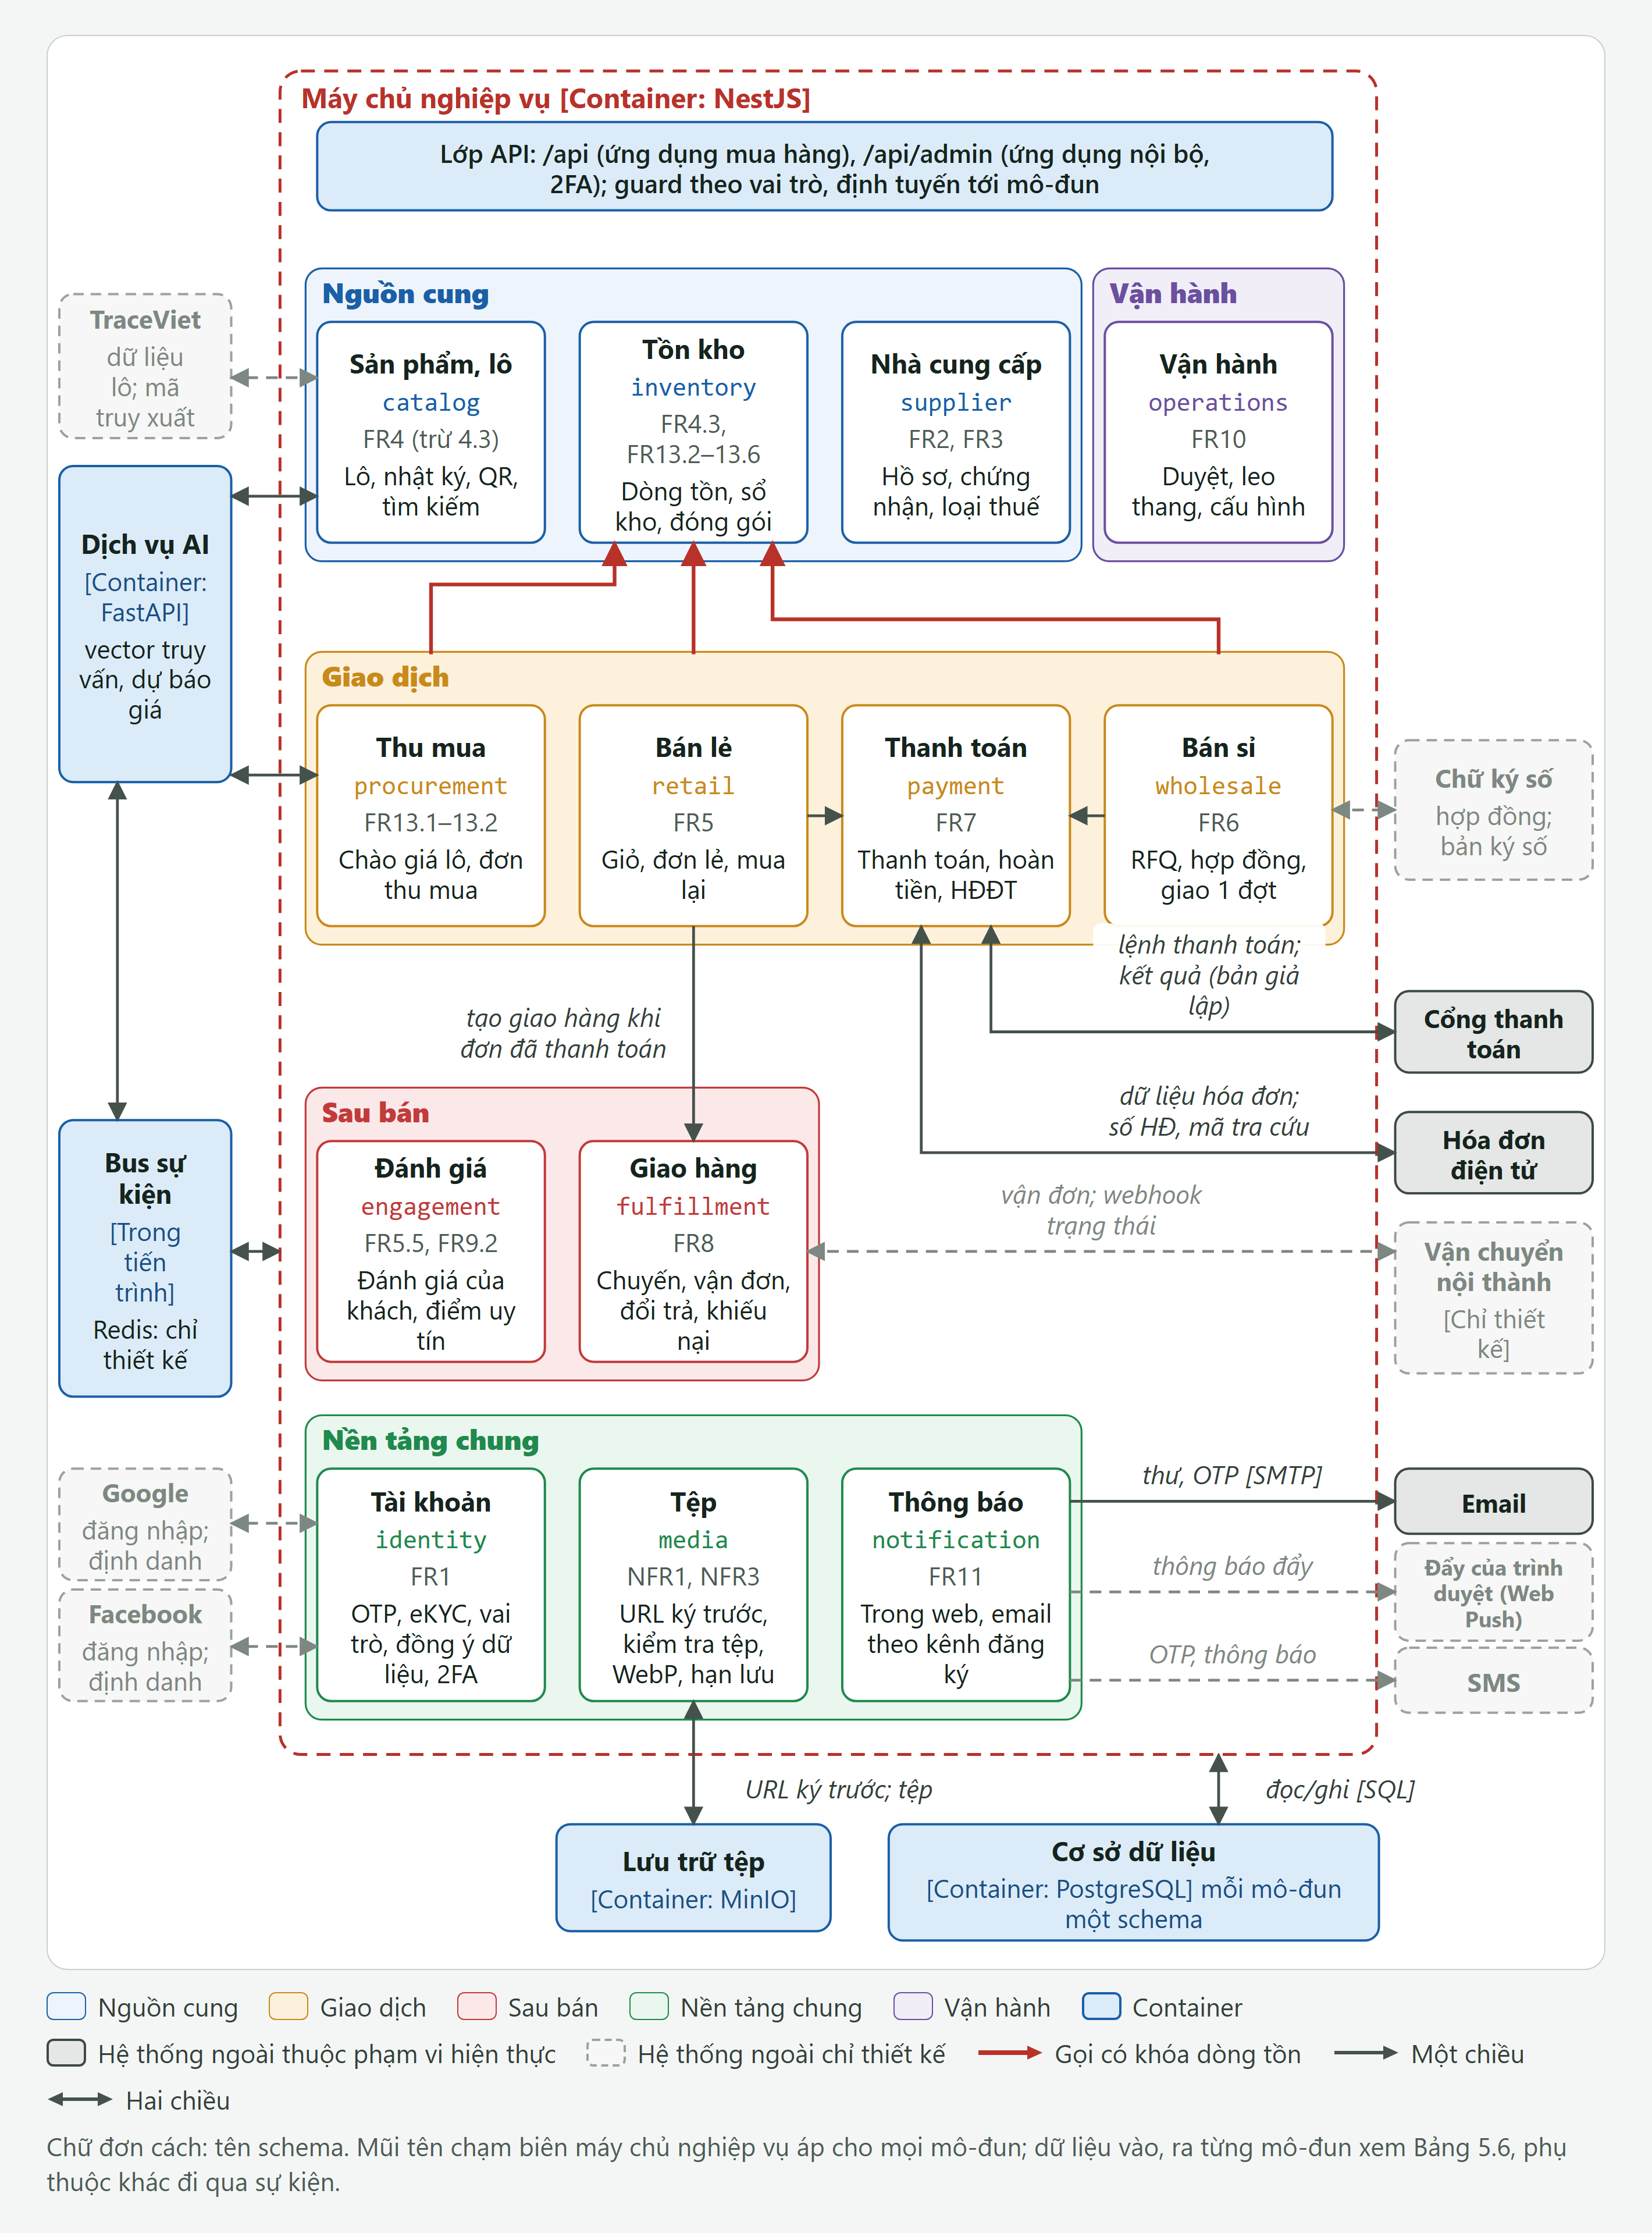
\includegraphics[width=\textwidth]{image/comparison/c4-module.png}
\end{adjustbox}
\caption{Các mô-đun của máy chủ nghiệp vụ (C4 mức 3)}
\label{fig:c4-module}
\end{figure}

\begingroup
\tblsetup\tblzebra
\begin{longtable}{L{1.55cm} L{2.40cm} L{5.00cm} L{2.85cm} L{2.40cm}}
\caption{Dữ liệu vào, ra và sự kiện của 13 mô-đun}
\label{tab:module-io} \\
\toprule
\rowcolor{tblheadbg}
\textbf{Khối} & \textbf{Mô-đun} & \textbf{Nhận vào $\rightarrow$ trả ra} & \textbf{Sự kiện phát} & \textbf{Gọi tới} \\
\midrule
\endfirsthead
\toprule
\rowcolor{tblheadbg}
\textbf{Khối} & \textbf{Mô-đun} & \textbf{Nhận vào $\rightarrow$ trả ra} & \textbf{Sự kiện phát} & \textbf{Gọi tới} \\
\midrule
\endhead
\bottomrule
\endfoot
Nền tảng chung & \texttt{identity} (FR1) & Hồ sơ đăng ký, OTP, eKYC, đồng ý dữ liệu $\rightarrow$ tài khoản, vai trò, phiên & \texttt{UserVerified} & \texttt{notification} \\
& \texttt{notification} (FR11) & Sự kiện đã đăng ký $\rightarrow$ thông báo web, email & --- & Email; Web Push, SMS \emph{(chỉ thiết kế)} \\
& \texttt{media} & Yêu cầu tải tệp $\rightarrow$ đường dẫn ký trước; ảnh WebP nhiều cỡ & --- & Lưu trữ tệp \\
Nguồn cung & \texttt{supplier} (FR2, FR3) & Hồ sơ, chứng nhận $\rightarrow$ hồ sơ đã duyệt, hạn hiệu lực & \texttt{CertExpired} & --- \\
& \texttt{catalog} (FR4) & Sản phẩm, lô, nhật ký; câu tìm kiếm $\rightarrow$ lô đã duyệt kèm QR, trang truy xuất, kết quả tìm & \texttt{BatchApproved}, \texttt{ProductChanged} & Dịch vụ AI \\
& \texttt{inventory} (FR4.3, FR13) & Lệnh giữ chỗ, trừ, nhập, đóng gói, thu hồi $\rightarrow$ dòng tồn, sổ nhập xuất & \texttt{StockLow}, \texttt{BatchRecalled} & --- \\
Giao dịch & \texttt{procurement} (FR13.1--13.2) & Chào giá lô, đơn thu mua, nghiệm thu $\rightarrow$ đơn đã xác nhận, nhập dòng tồn & \texttt{ProcurementReceived} & \texttt{inventory} \\
& \texttt{retail} (FR5) & Giỏ, đơn lẻ, mua lại $\rightarrow$ đơn kèm dòng thời gian tám trạng thái & \texttt{OrderPlaced}, \texttt{OrderCancelled} & \texttt{inventory}, \texttt{payment}, \texttt{fulfillment} \\
& \texttt{wholesale} (FR6) & RFQ, báo giá, xác nhận giao kết $\rightarrow$ hợp đồng kèm mã băm, đơn sỉ & \texttt{RfqUpdated}, \texttt{ContractConcluded} & \texttt{identity}, \texttt{media}, \texttt{inventory}, \texttt{payment} \\
& \texttt{payment} (FR7) & Lệnh thanh toán, hoàn tiền $\rightarrow$ trạng thái thanh toán, hóa đơn giả lập, đối soát sỉ & \texttt{PaymentSucceeded}, \texttt{Refunded} & Cổng thanh toán, hóa đơn (giả lập) \\
Sau bán & \texttt{fulfillment} (FR8, FR9.1) & Đơn đã thanh toán, chuyến trung chuyển, yêu cầu đổi trả $\rightarrow$ vận đơn, trạng thái giao, quyết định khiếu nại & \texttt{ShipmentStatusChanged}, \texttt{CaseResolved} & Đơn vị vận chuyển \emph{(chỉ thiết kế)} \\
& \texttt{engagement} (FR5.5, FR9.2) & Đánh giá sau đơn hoàn tất $\rightarrow$ điểm đánh giá, điểm uy tín & \texttt{ReviewPosted} & \texttt{retail} \\
Vận hành & \texttt{operations} (FR10) & Quyết định duyệt, khóa, thu hồi; cấu hình $\rightarrow$ hàng đợi duyệt, nhật ký thao tác, bảng điều khiển & --- & \texttt{catalog}, \texttt{supplier}, \texttt{inventory}, \texttt{engagement} \\
\end{longtable}
\endgroup

\noindent\textbf{Quyết định kiến trúc đáng chú ý.} (i) \emph{Giữ chỗ trước, trừ tồn sau:} khi đặt đơn ở bất kỳ luồng nào, hệ thống khóa dòng tồn trong một giao dịch, kiểm tra số lượng còn rồi mới giữ chỗ 15 phút; chỉ khi có \texttt{PaymentSucceeded} hoặc COD đủ điều kiện mới chuyển thành trừ tồn --- đó là lý do tồn kho và đơn hàng phải chung một cơ sở dữ liệu. (ii) \emph{Sự kiện đi qua một cổng phát sự kiện} (bản hiện thực chạy trong tiến trình, Redis \emph{chỉ thiết kế}) cho thông báo, cập nhật dòng thời gian, vòng phản hồi AI, nên mô-đun nhận chậm không làm chậm người dùng và việc chuyển sang Redis hay message broker chuyên dụng về sau không phải sửa mã phát sự kiện. (iii) \emph{Kết quả từ bên ngoài được xử lý một lần} (theo thiết kế đi vào qua webhook \emph{(chỉ thiết kế)}): cổng thanh toán gửi lại cùng kết quả thì trạng thái đơn không đổi thêm. (iv) \emph{Trang truy xuất công khai} chỉ đọc, cache tích cực và tách khỏi vùng cần xác thực vì có thể bị quét dồn dập; đây là thành phần nên tách ra trước nếu hệ thống cần chia nhỏ.

\subsection{Thiết kế sitemap}
\label{sec:sitemap}

Sitemap thể hiện tổ chức trang theo cấp bậc~\cite{nngroup_sitemap}, bắc cầu giữa use case (người dùng làm được gì) và thiết kế giao diện; Hình~\ref{fig:sitemap} trình bày hai cấp đầu. Ứng dụng mua hàng có bốn khu theo luồng nghiệp vụ (công khai kèm đăng ký, đăng nhập; khách lẻ; khách sỉ; nhà cung cấp), trục bán lẻ đi trọn từ tìm kiếm, chi tiết, giỏ, thanh toán tới đơn hàng, đổi trả, đánh giá. Ứng dụng nội bộ có sáu mục theo vai trò, mỗi người chỉ thấy mục của vai trò mình. Không có trang tin nhắn chung: trao đổi gắn với đơn hoặc yêu cầu đổi trả (FR9.1, \emph{chỉ thiết kế}). Trang chỉ thiết kế vẽ xám nét đứt. Sitemap độc lập framework: khi hiện thực, mỗi khu ứng với một nhóm route có bố cục và kiểm tra đăng nhập riêng.

\begin{figure}[H]
\centering
\begin{adjustbox}{max totalsize={\textwidth}{0.62\textheight},center}
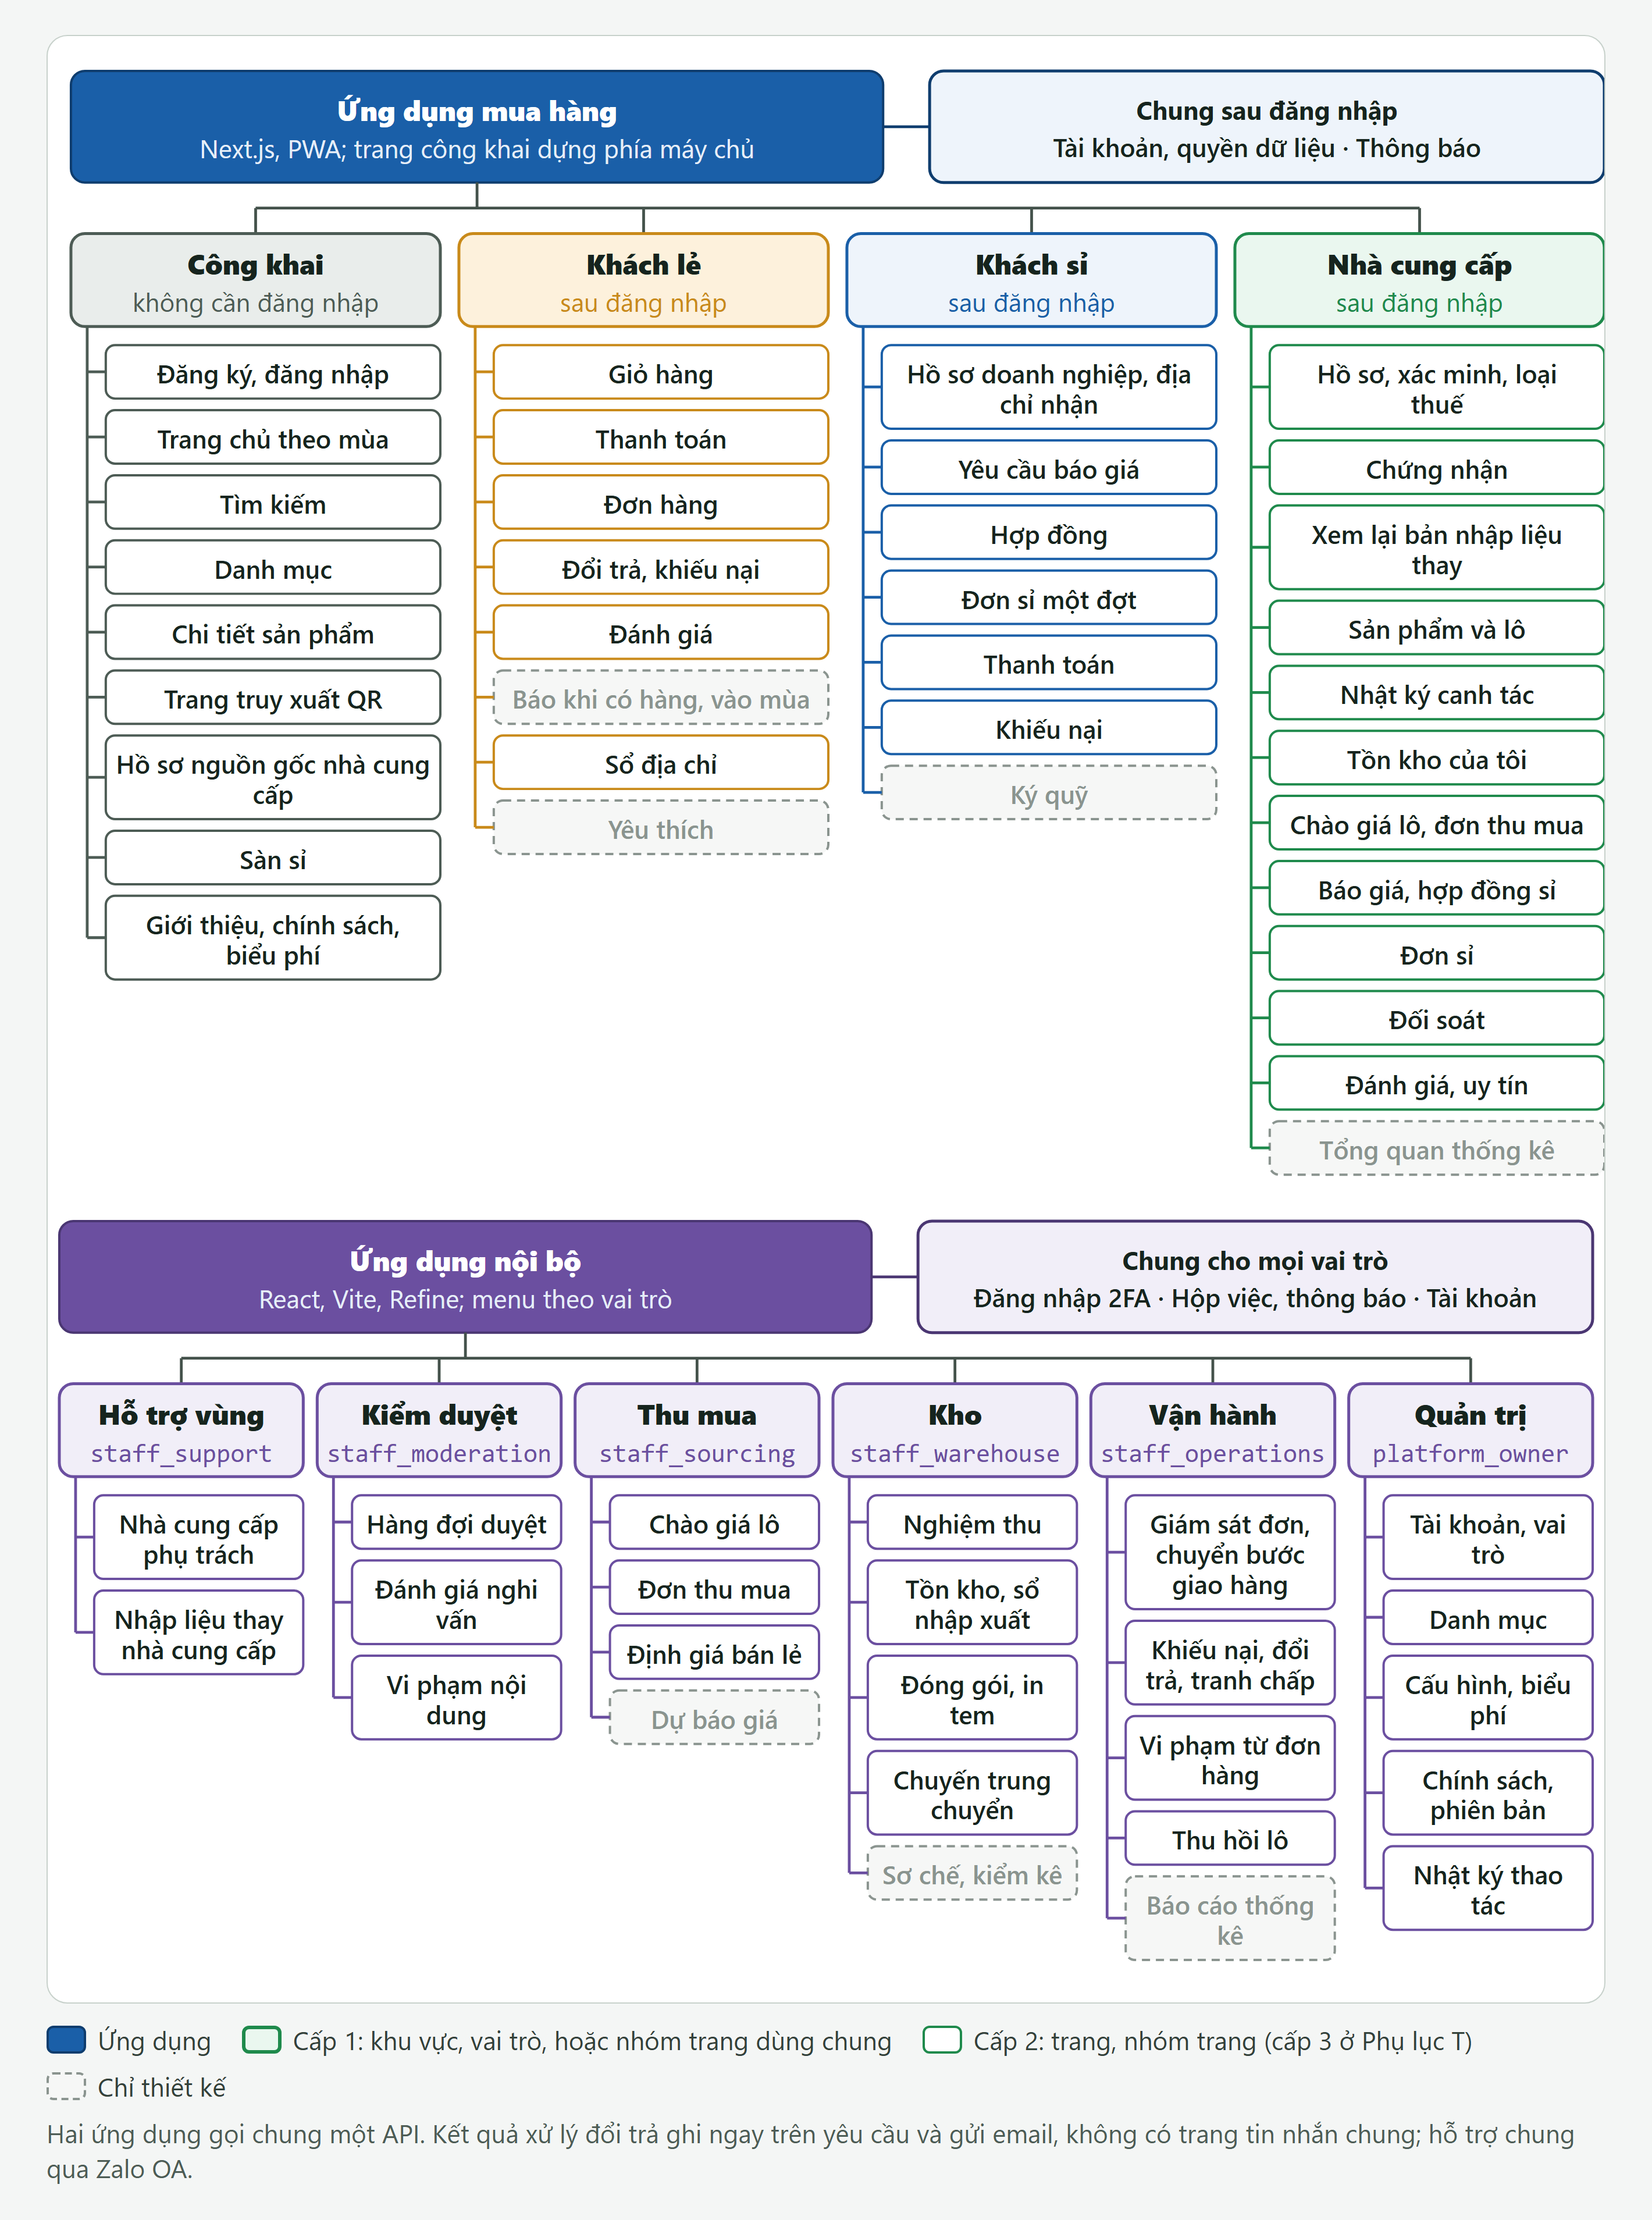
\includegraphics[width=\textwidth]{image/comparison/sitemap-tong-quan.png}
\end{adjustbox}
\caption{Sitemap tổng quan của hai ứng dụng Farmery (cấp 1 và 2)}
\label{fig:sitemap}
\end{figure}

\subsection{Thiết kế lược đồ tuần tự}
\label{subsec:tuantu}

Lược đồ tuần tự đi sâu hơn ở mức mô-đun: tách lời gọi khỏi giá trị trả về, vẽ nhánh loại trừ bằng khung \texttt{alt}, lặp bằng \texttt{loop}; mỗi đường đời là một mô-đun của Bảng~\ref{tab:module-io}, người dùng hoặc hệ thống bên ngoài; sự kiện qua bus sự kiện vẽ nét đứt màu tím. Hai luồng có nhiều mô-đun phối hợp nhất được chọn: đặt hàng và thanh toán đơn lẻ (Hình~\ref{fig:seq-dat-hang}) với ba nhánh trả trước thành công, COD đủ điều kiện, thất bại hoặc quá 15 phút; và từ yêu cầu báo giá đến xác nhận giao kết hợp đồng sỉ (Hình~\ref{fig:seq-hop-dong-si}), nơi báo giá được chấp nhận sinh hợp đồng có mã băm và mỗi bên xác nhận bằng OTP qua email. Qua hai lược đồ thấy rõ: mọi lời gọi cần kết quả ngay (giữ chỗ, trừ tồn, kiểm OTP) nằm trong cùng giao dịch, còn thông báo và cập nhật dòng thời gian đi qua sự kiện.

\begin{figure}[H]
\centering
\begin{adjustbox}{max totalsize={\textwidth}{0.62\textheight},center}
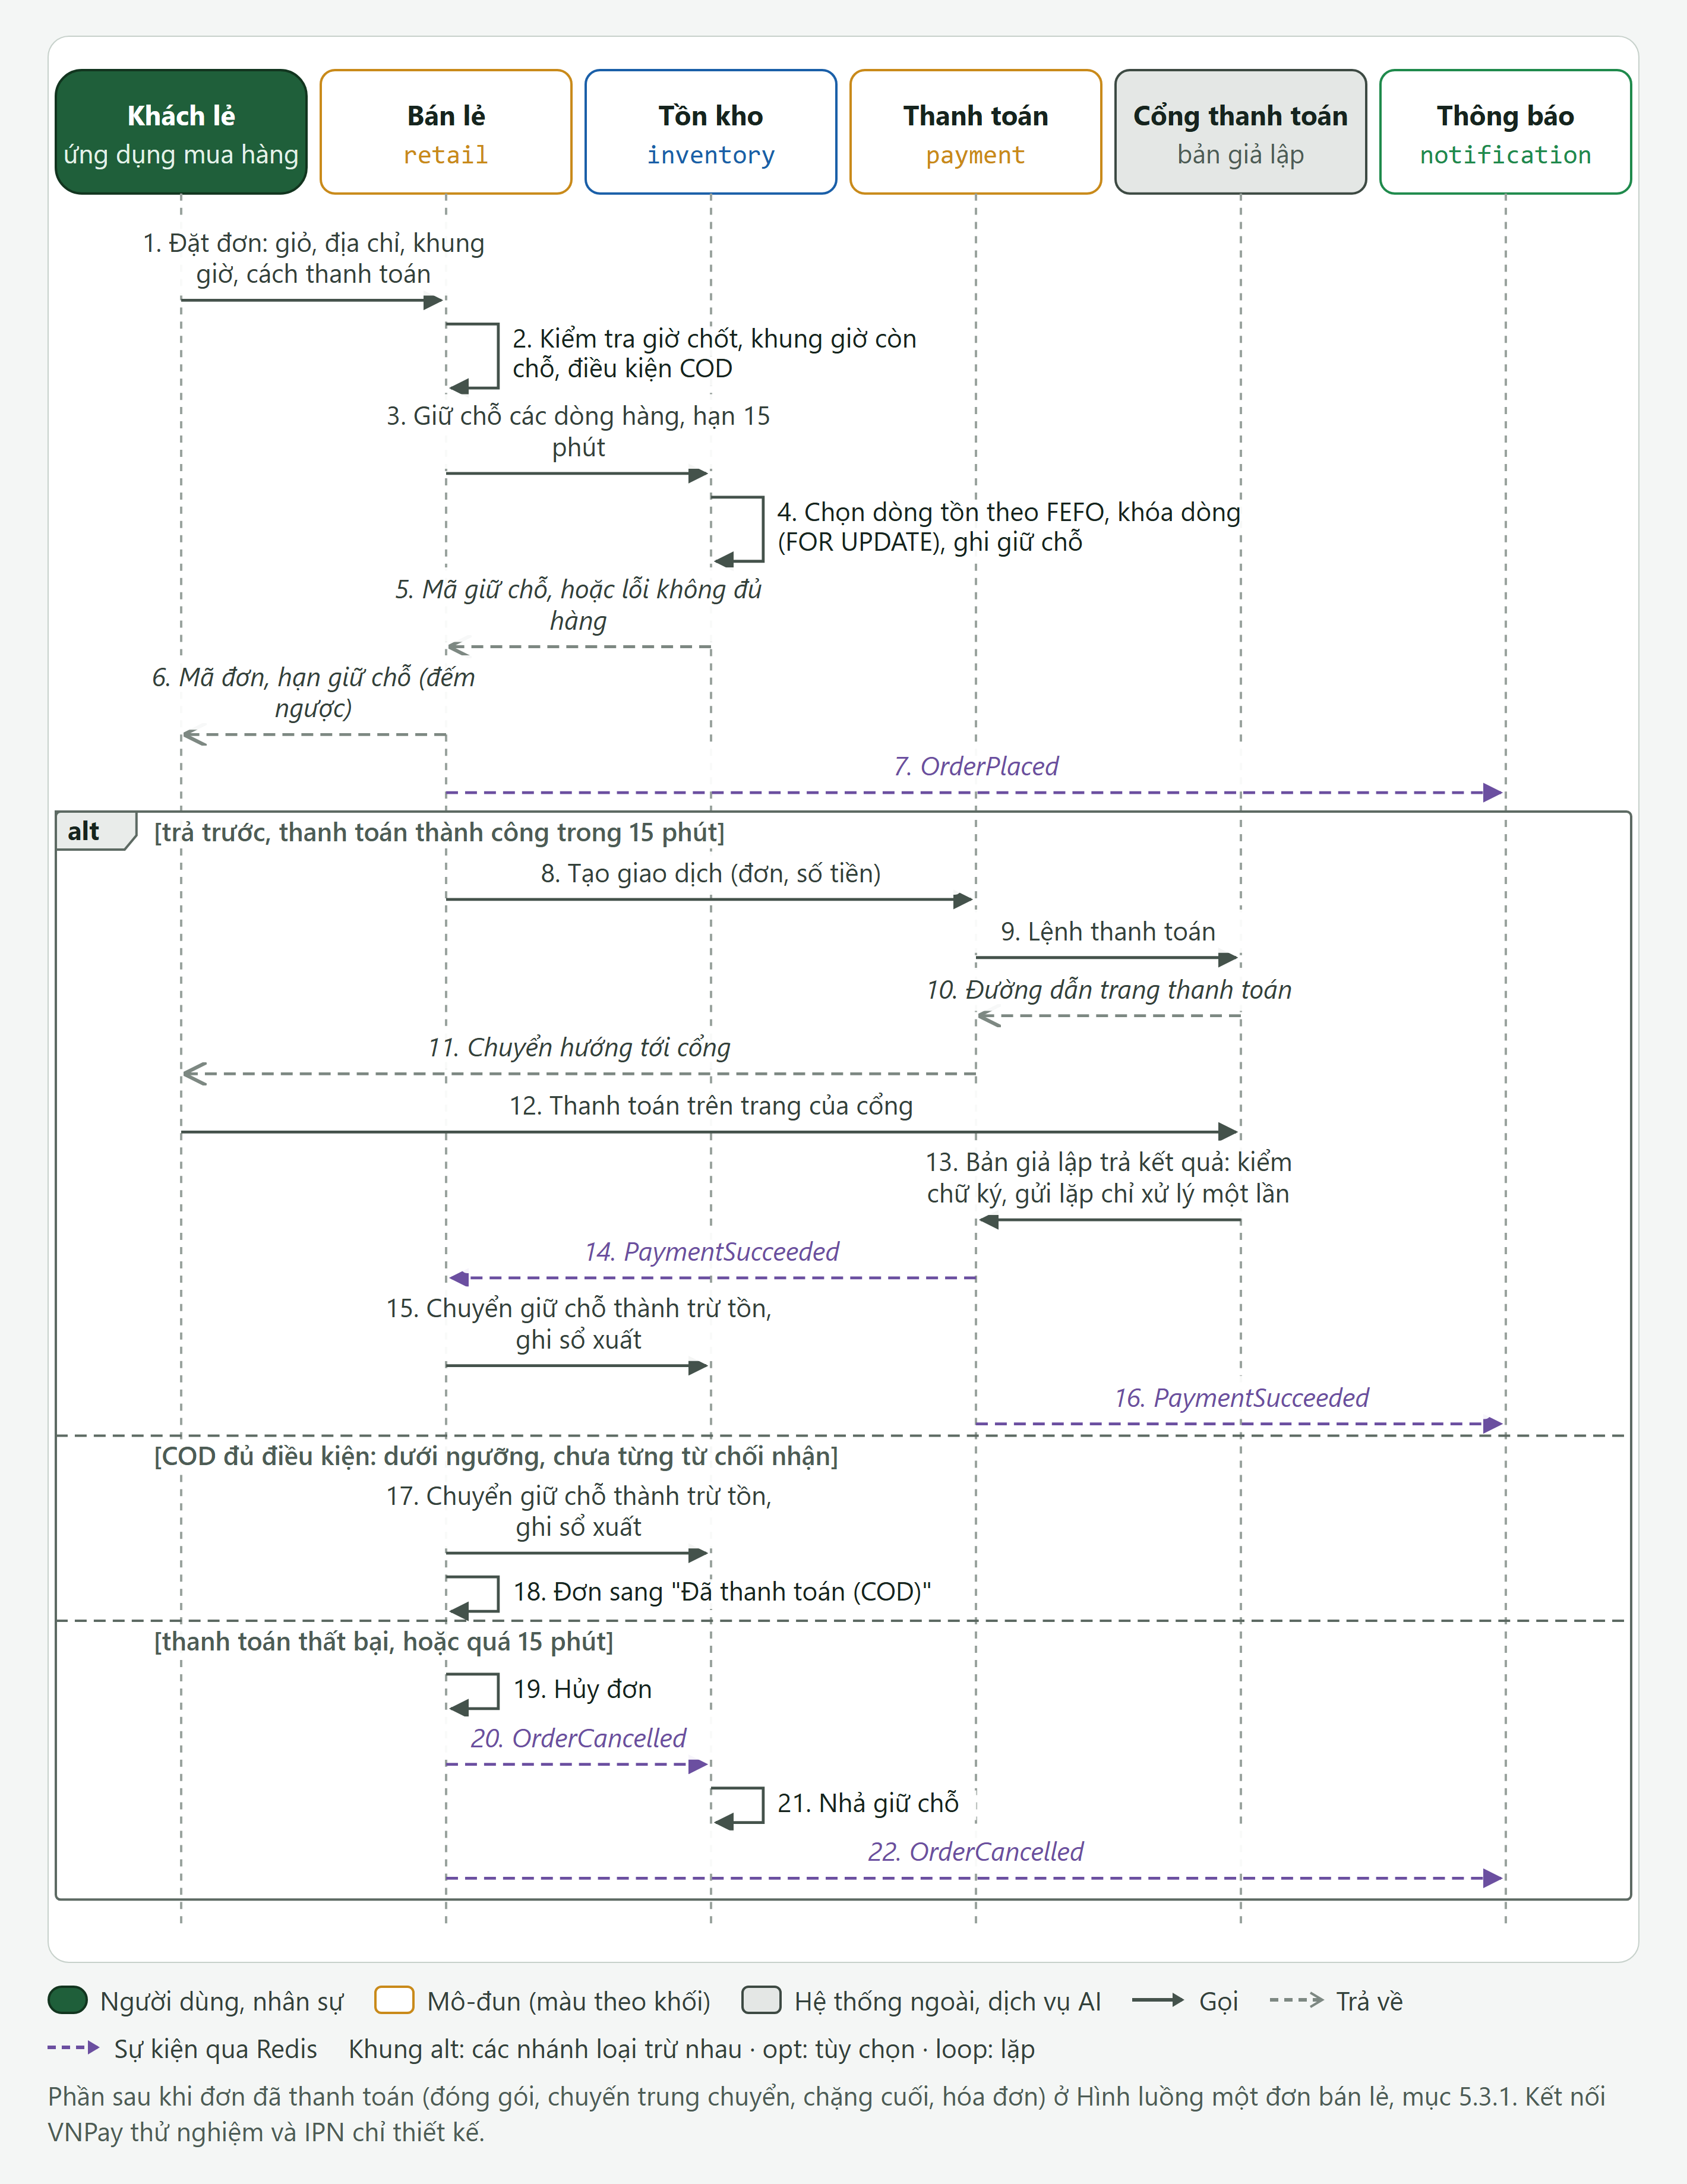
\includegraphics[width=\textwidth]{image/comparison/seq-dat-hang.png}
\end{adjustbox}
\caption{Lược đồ tuần tự đặt hàng và thanh toán đơn lẻ}
\label{fig:seq-dat-hang}
\end{figure}

\begin{figure}[H]
\centering
\begin{adjustbox}{max totalsize={\textwidth}{0.62\textheight},center}
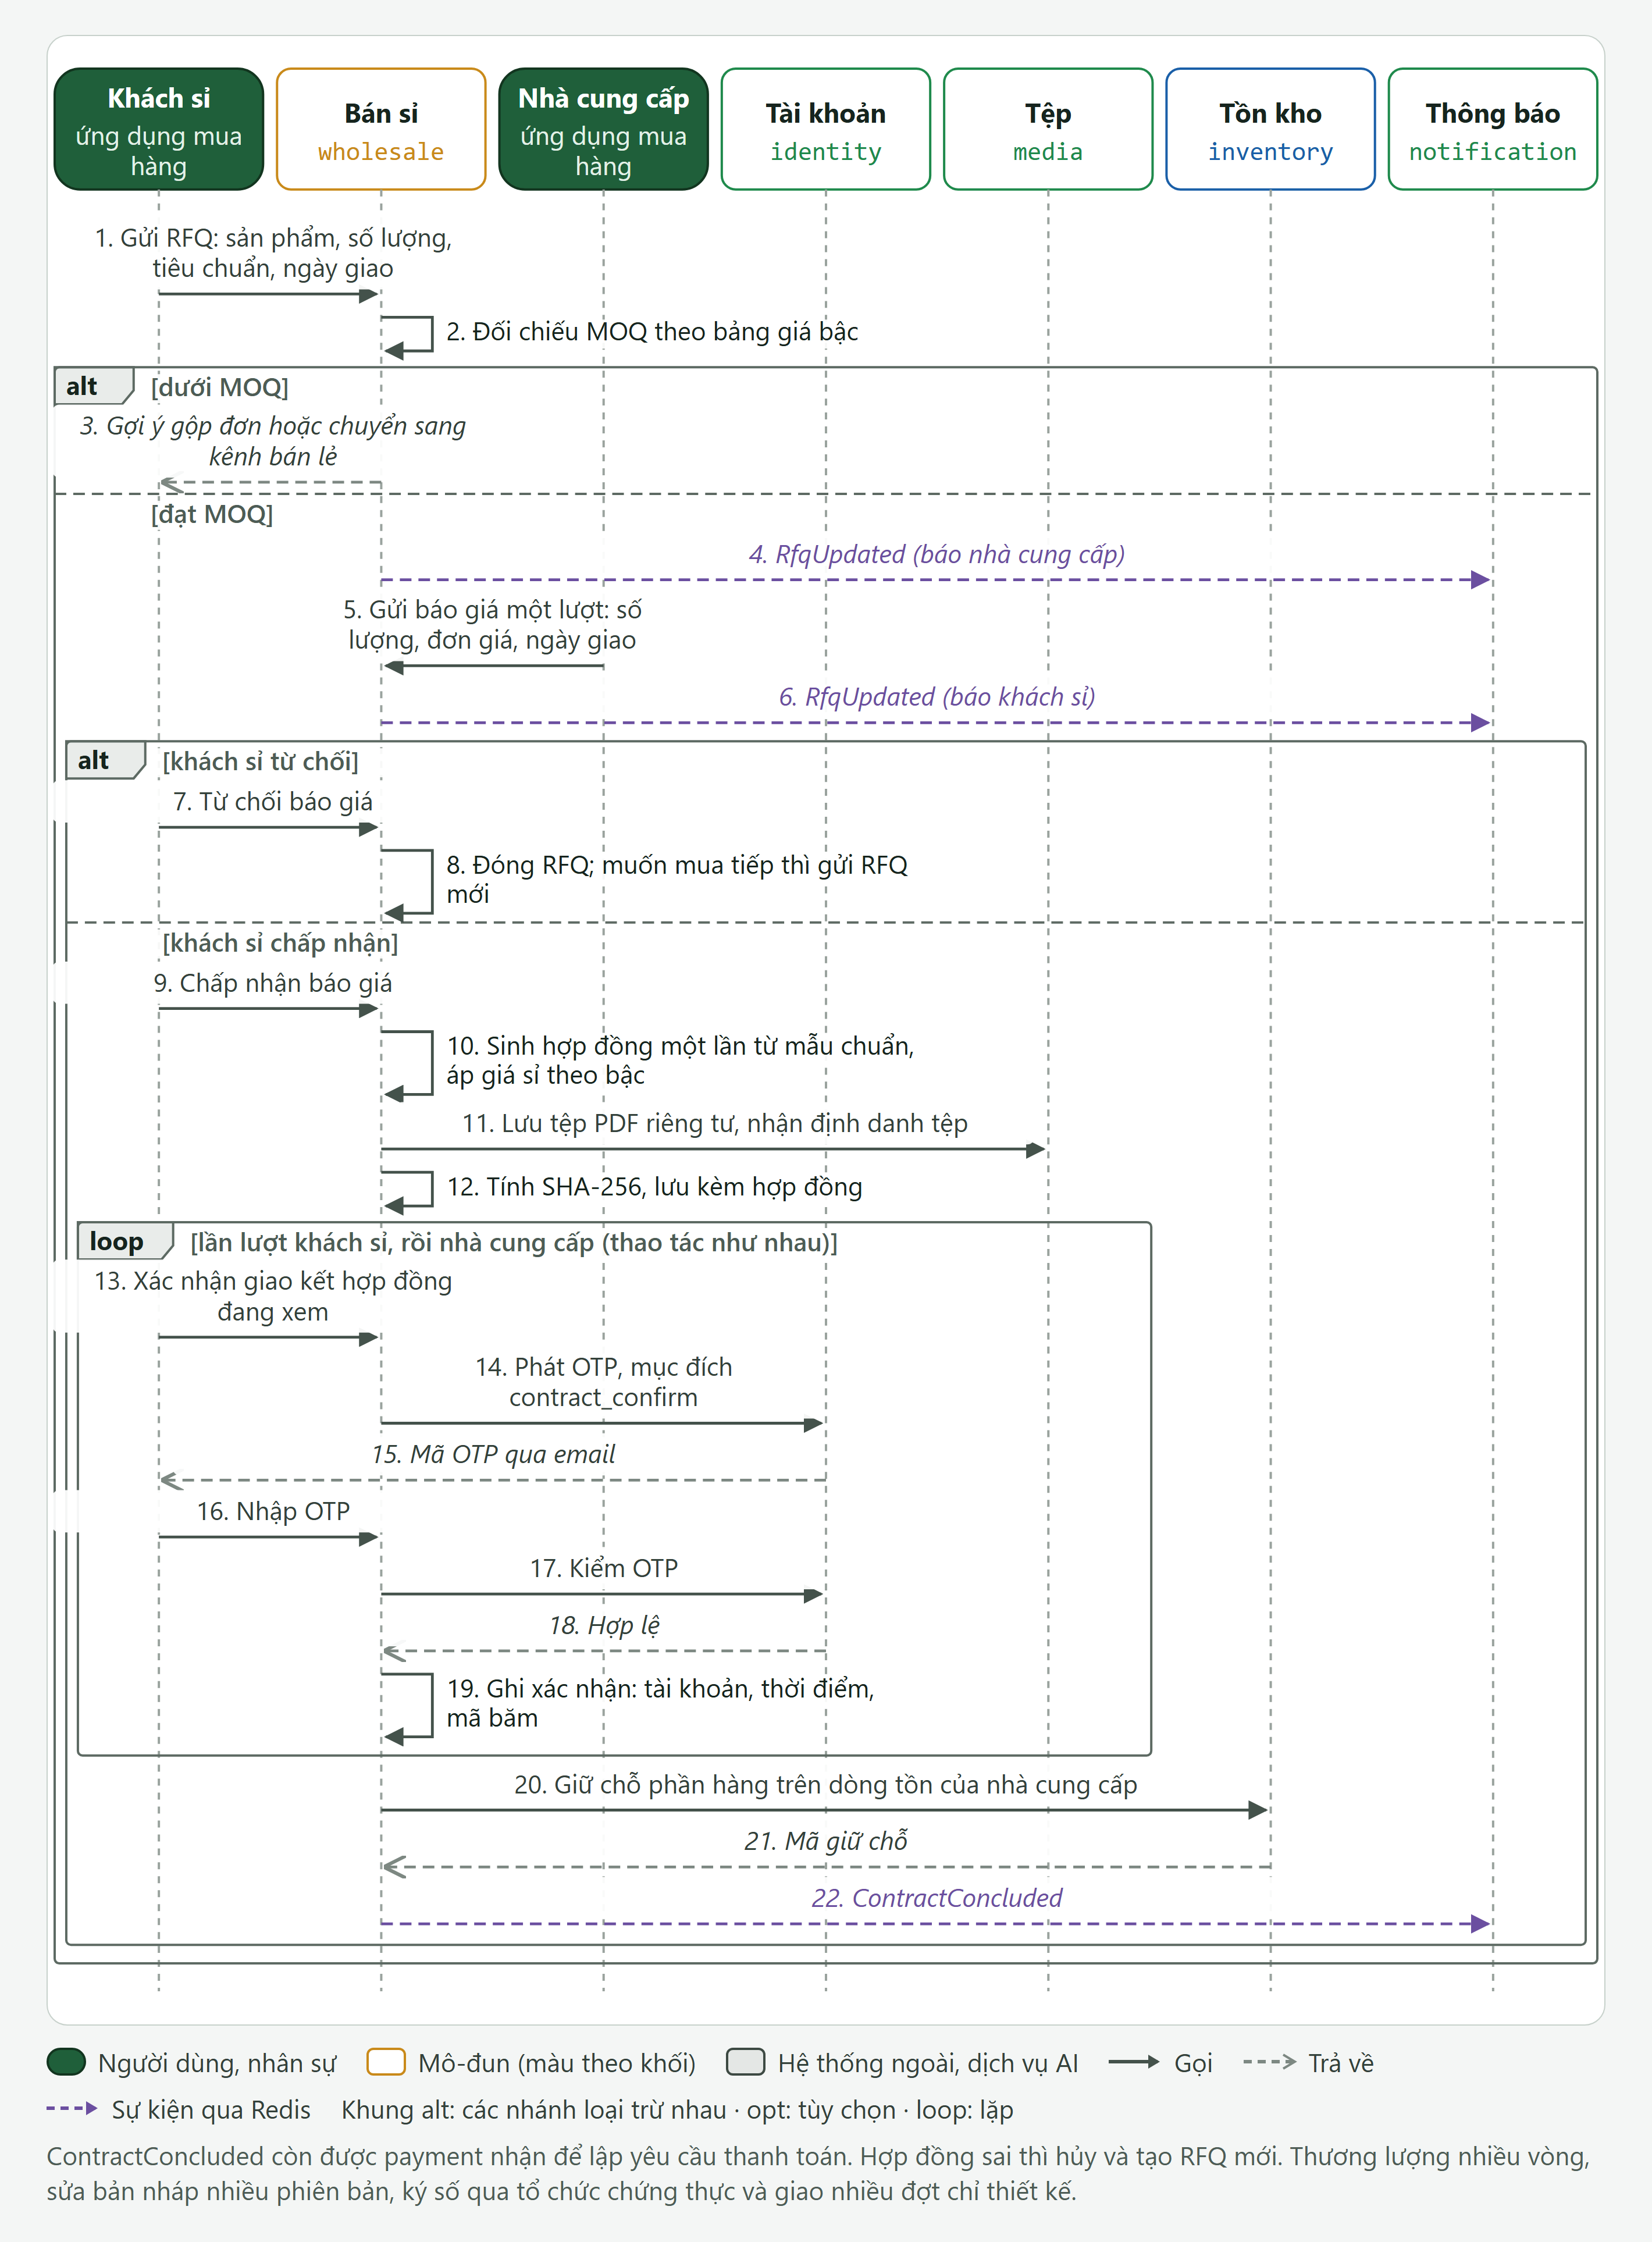
\includegraphics[width=\textwidth]{image/comparison/seq-hop-dong-si.png}
\end{adjustbox}
\caption{Lược đồ tuần tự từ yêu cầu báo giá đến xác nhận giao kết hợp đồng sỉ}
\label{fig:seq-hop-dong-si}
\end{figure}

\subsection{Thiết kế lược đồ lớp}
\label{subsec:lop}

Hình~\ref{fig:class-mien} trình bày các lớp miền của trục bán lẻ và phần nguồn cung đứng trước nó (đúng phạm vi hiện thực ở mục~\ref{sec:phamvi}); mỗi lớp ứng với một bảng cùng tên (mục~\ref{sec:csdl}) và thuộc đúng một mô-đun. Phương thức là thao tác nghiệp vụ chứ không phải hàm đọc ghi trường: đơn chỉ đổi trạng thái qua \texttt{advance}, \texttt{cancel}, \texttt{complete}; dòng tồn chỉ đổi qua \texttt{reserve} rồi \texttt{consume} hoặc \texttt{release}, nên ràng buộc không bán vượt, không nhảy cóc trạng thái nằm ở một chỗ. Quan hệ hợp thành (hình thoi đặc) khi lớp con không tồn tại tách khỏi lớp chứa; liên kết xuyên mô-đun vẽ nét đứt vì hai lớp chỉ giữ định danh của nhau (RB3), ví dụ \texttt{OrderItem} lưu \texttt{holdingId} và \texttt{batchId}.

\begin{figure}[H]
\centering
\begin{adjustbox}{max totalsize={\textwidth}{0.62\textheight},center}
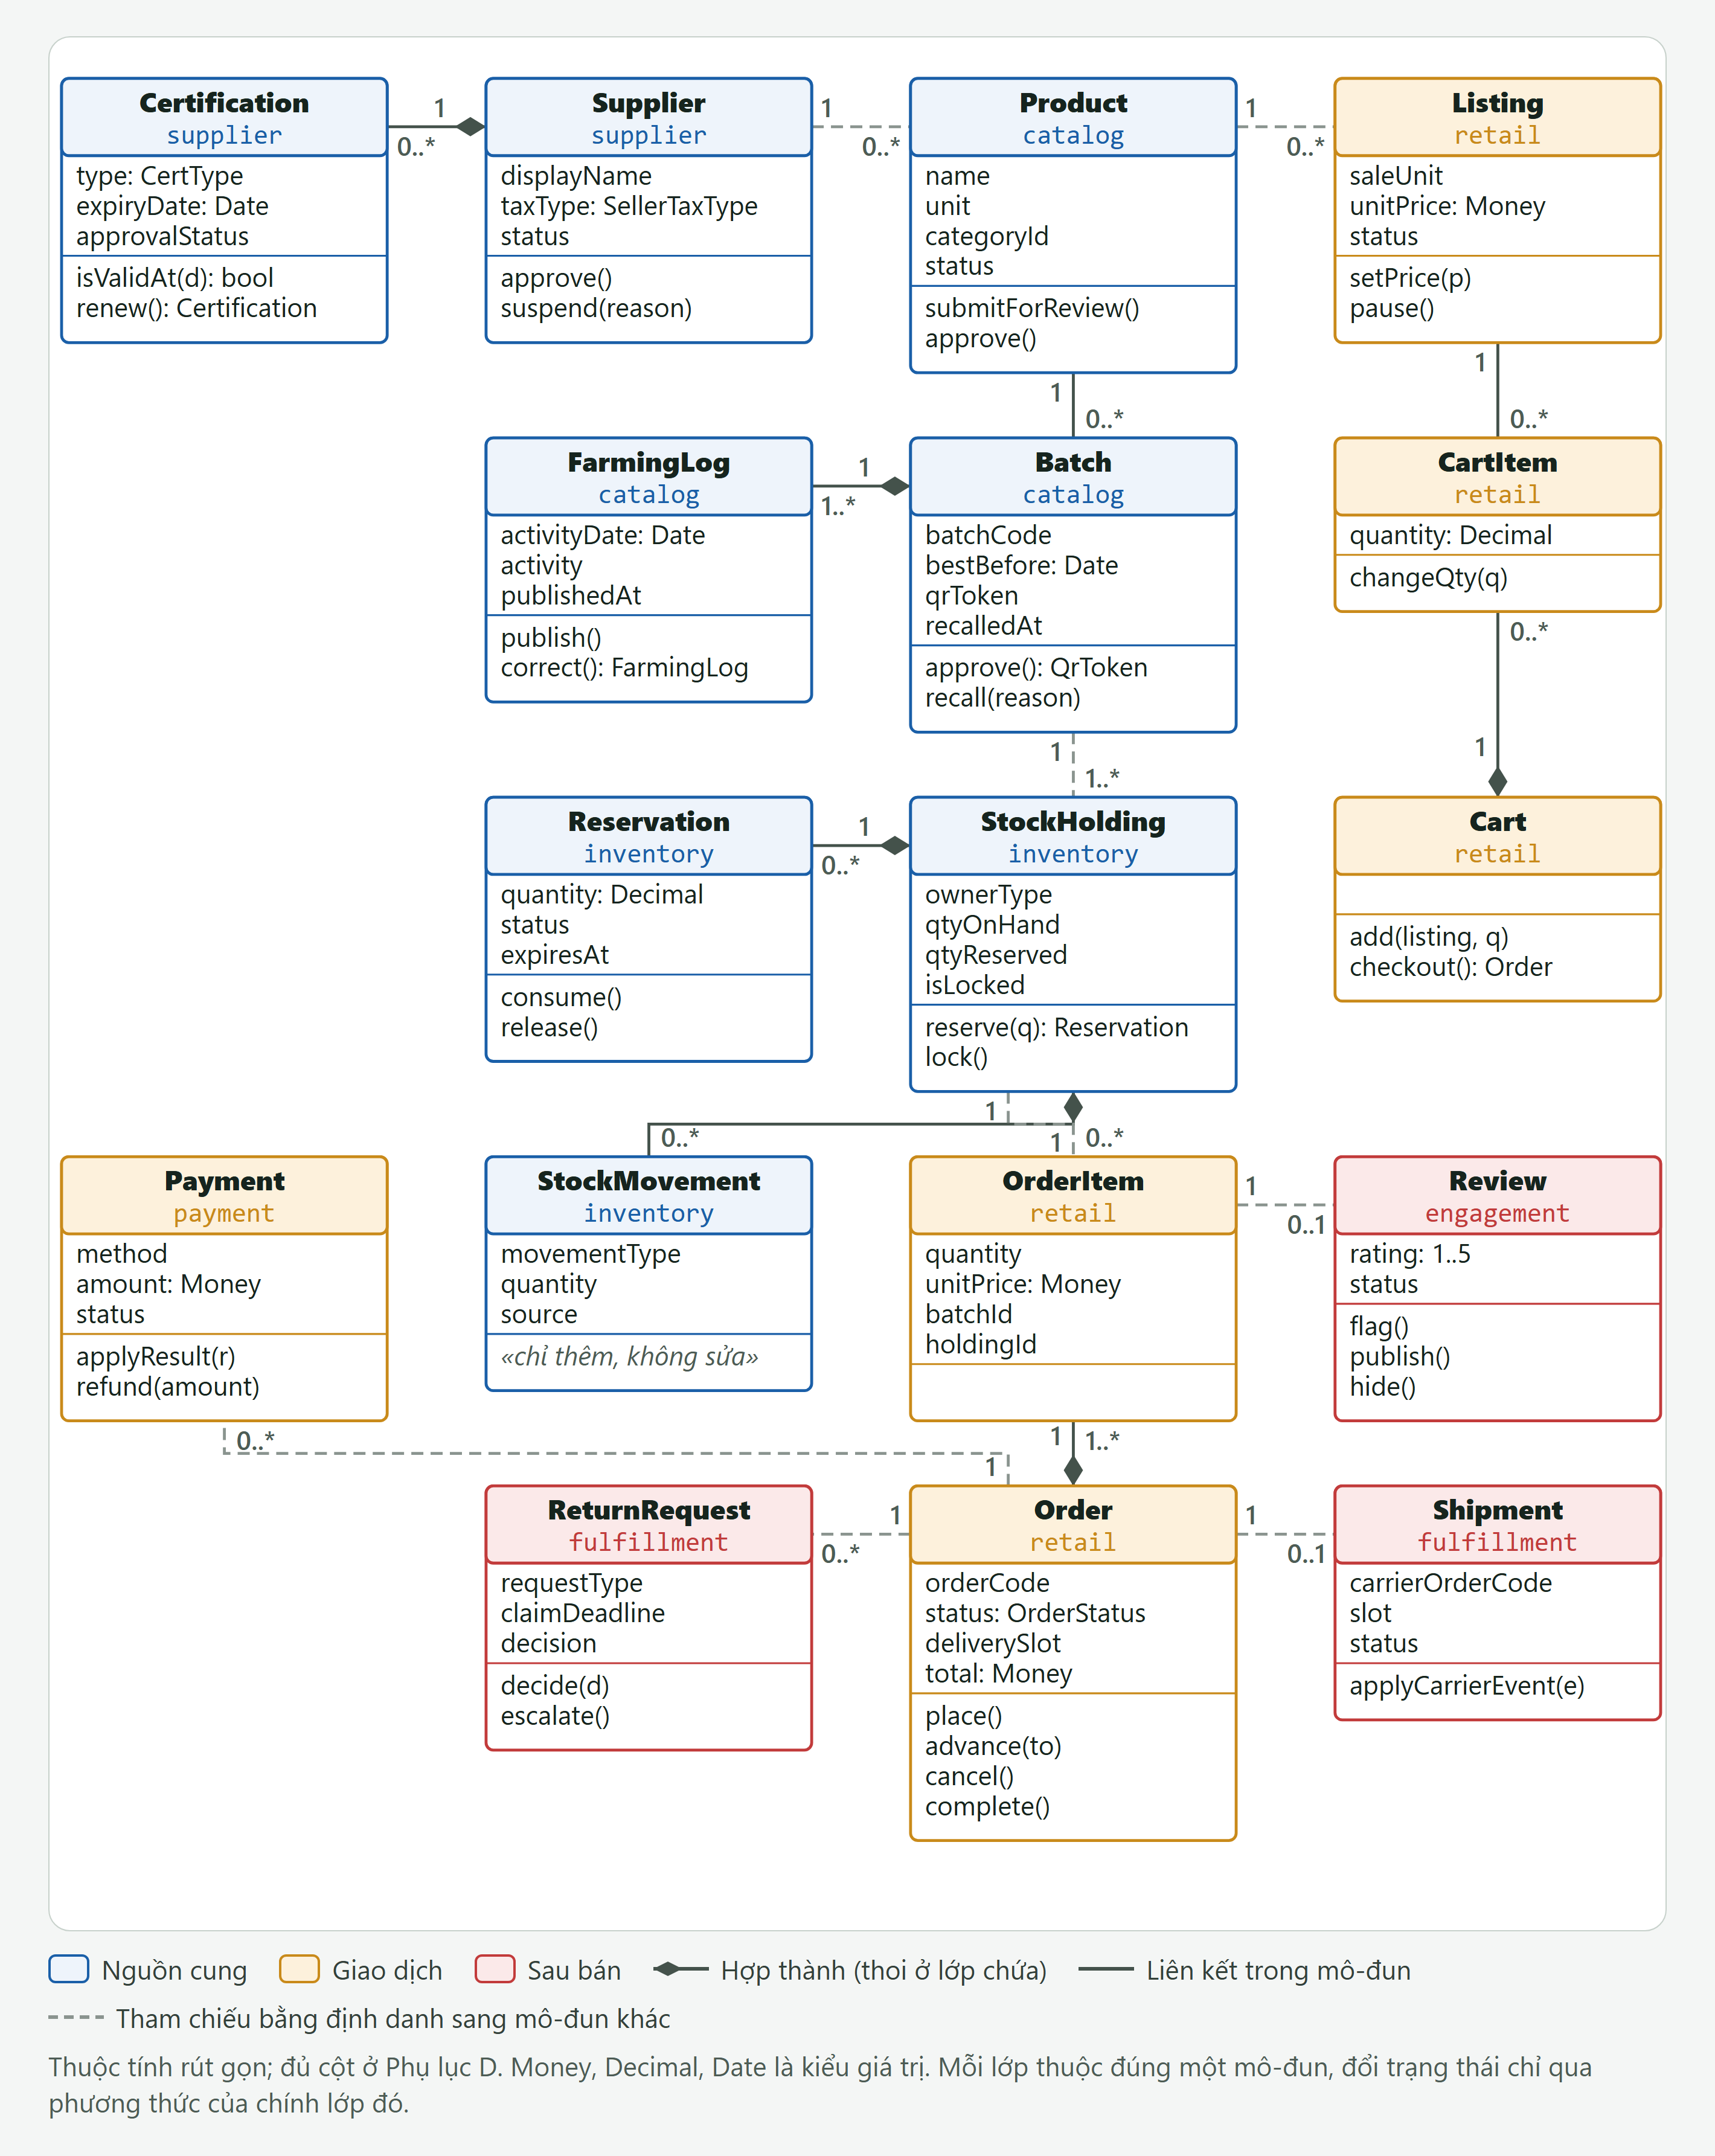
\includegraphics[width=\textwidth]{image/comparison/class-mien.png}
\end{adjustbox}
\caption{Lược đồ lớp miền của trục bán lẻ và nguồn cung}
\label{fig:class-mien}
\end{figure}

\subsection{Thiết kế cơ sở dữ liệu}
\label{sec:csdl}

\label{subsec:dacta-csdl}
Cơ sở dữ liệu gồm 13 schema trùng tên và ranh giới với 13 mô-đun (Bảng~\ref{tab:module-io}), tổng 65 bảng, 565 cột, 48 khóa ngoại; mỗi mô-đun sở hữu đúng một schema và tham chiếu sang schema khác bằng định danh, không kết nối xuyên schema (RB3). Theo năm khối: \emph{nền tảng chung} (\texttt{identity}: tài khoản, vai trò, địa chỉ, hồ sơ doanh nghiệp, eKYC, đồng ý dữ liệu; \texttt{notification}; \texttt{media}: tệp kèm mã băm, mức truy cập, hạn lưu); \emph{nguồn cung} (\texttt{supplier}: hồ sơ, chứng nhận; \texttt{catalog}: danh mục, sản phẩm, lô, nhật ký, QR, vector; \texttt{inventory}: dòng tồn, sổ nhập xuất, giữ chỗ, thu hồi); \emph{giao dịch} (\texttt{procurement}, \texttt{retail}, \texttt{wholesale}, \texttt{payment}); \emph{sau bán} (\texttt{fulfillment}, \texttt{engagement}); \emph{vận hành} (\texttt{operations}: cấu hình, hàng đợi duyệt, vi phạm, nhật ký thao tác). Mô tả từng bảng và sơ đồ ERD chi tiết từng miền ở Phụ lục~D, danh sách đầy đủ từng cột trong tệp \texttt{schema.dbml}; tất cả sinh tự động từ cùng tệp lược đồ của dự án nên không lệch nhau.

Hình~\ref{fig:erd-tong-quan} là ma trận phụ thuộc giữa các schema: mỗi hàng là schema có cột tham chiếu, mỗi cột là schema được tham chiếu, số trong ô là số cột tham chiếu xuyên schema (\texttt{identity} và \texttt{media} không đưa vào cột vì gần như mọi schema đều tham chiếu). Trong các ERD chi tiết, nét liền là khóa ngoại thật trong cùng schema, nét đứt là tham chiếu xuyên schema bằng định danh (phản ánh trực tiếp RB3), bảng chỉ thiết kế vẽ nét đứt nền xám.

\begin{figure}[H]
\centering
\begin{adjustbox}{max totalsize={\textwidth}{0.62\textheight},center}
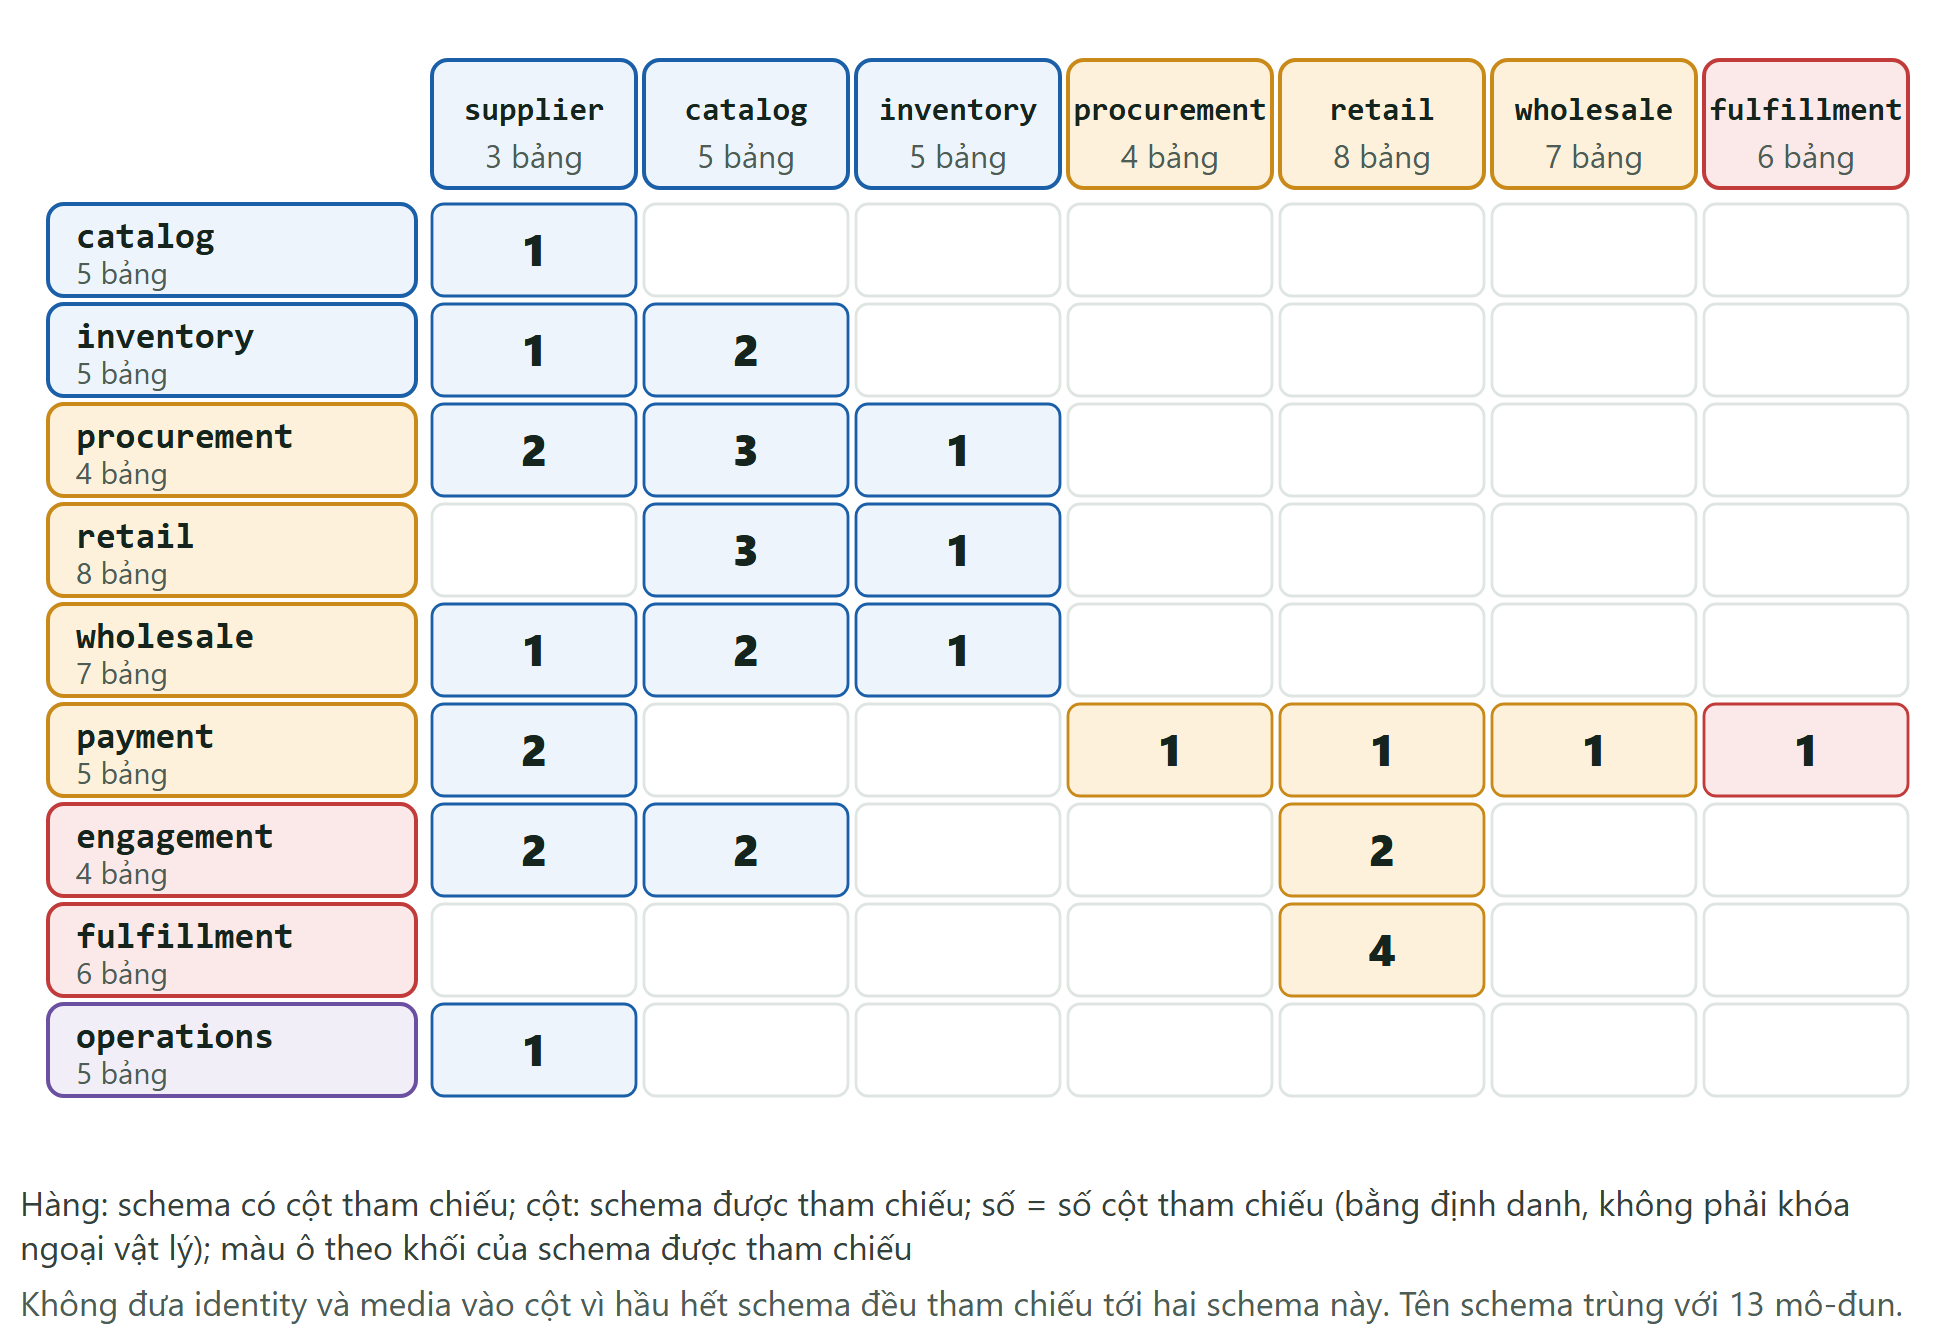
\includegraphics[width=\textwidth]{image/comparison/erd-tong-quan.png}
\end{adjustbox}
\caption{ERD tổng quan: ma trận phụ thuộc giữa các schema (số ô là số cột tham chiếu xuyên schema)}
\label{fig:erd-tong-quan}
\end{figure}

\noindent\textbf{Ánh xạ ERD sang lược đồ quan hệ.} Lược đồ quan hệ suy ra từ ERD theo các quy tắc sau; Phụ lục~\ref{apdx:quanhe} (Bảng~\ref{tab:luocdoquanhe}) viết đủ 65 bảng theo dạng \emph{bảng}(\underline{khóa chính}, \emph{khóa ngoại}$\rightarrow$bảng cha, thuộc tính).
\begin{itemize}
    \item \textbf{Thực thể và thuộc tính:} mỗi thực thể thành một bảng, mỗi thuộc tính thành một cột; khóa chính thường là cột \texttt{id} kiểu \texttt{bigint} tự tăng.
    \item \textbf{Quan hệ 1--N:} khóa ngoại nằm ở bảng phía N và là ràng buộc vật lý khi hai bảng cùng schema (48 khóa ngoại), ví dụ \texttt{order\_items.order\_id} trỏ tới \texttt{orders}.
    \item \textbf{Quan hệ N--N:} thành bảng nối có khóa chính ghép từ hai khóa ngoại (7 bảng), ví dụ \texttt{user\_roles}(\underline{user\_id}, \underline{role}) cho một người nhiều vai trò, \texttt{cart\_items}(\underline{cart\_id}, \underline{listing\_id}) cho giỏ hàng.
    \item \textbf{Quan hệ 1--1:} khóa ngoại kèm ràng buộc duy nhất, ví dụ mỗi đơn có một vận đơn (\texttt{shipments.order\_id}), mỗi chủ một doanh nghiệp (\texttt{businesses.owner\_user\_id}).
    \item \textbf{Tham chiếu xuyên schema (92 cột):} chỉ lưu định danh, không tạo khóa ngoại vật lý (ràng buộc RB3), vẽ bằng nét đứt trên ERD; toàn vẹn tham chiếu do tầng ứng dụng của mô-đun sở hữu bảo đảm.
    \item \textbf{Cột mảng và kiểu liệt kê:} danh sách định danh tệp lưu thành cột mảng (8 cột như \texttt{image\_ids}) thay vì bảng nối; trạng thái và loại lưu bằng 41 kiểu liệt kê của PostgreSQL.
\end{itemize}
Chiến lược chỉ mục ở mục I.2 của Phụ lục~\ref{apdx:quanhe}: chỉ mục đã có trong migration (27 ràng buộc duy nhất và 3 chỉ mục tìm kiếm) và 14 chỉ mục đề xuất theo truy vấn, chưa khai trong \texttt{schema.prisma}.

\subsection{Thiết kế mô-đun AI}
\label{sec:thietkeAI}

Cả ba mô-đun AI (Chương~\ref{chap:coso}) đi theo một luồng chung năm bước: \emph{thu thập} sự kiện từ quy trình nghiệp vụ (lượt xem, mua, đơn, đánh giá, hủy đơn); \emph{tiền xử lý} và trích đặc trưng; \emph{huấn luyện và suy luận} (dự báo giá tính lại theo lô định kỳ; vector sản phẩm tính khi sản phẩm được duyệt hoặc sửa mô tả; tìm kiếm và sản phẩm tương tự suy luận trực tuyến); \emph{phục vụ kết quả} qua API nội bộ (trang kết quả tìm kiếm, trang sản phẩm; màn hình thu mua \emph{(chỉ thiết kế)}); \emph{vòng phản hồi} ghi nhận phản ứng của người dùng để bổ sung tập đánh giá. Hình~\ref{fig:ai-luong} vẽ luồng này cho từng tính năng và Bảng~\ref{tab:tinhnangAI} cụ thể hóa thêm.

\begin{figure}[H]
\centering
\begin{adjustbox}{max totalsize={\textwidth}{0.5\textheight},center}
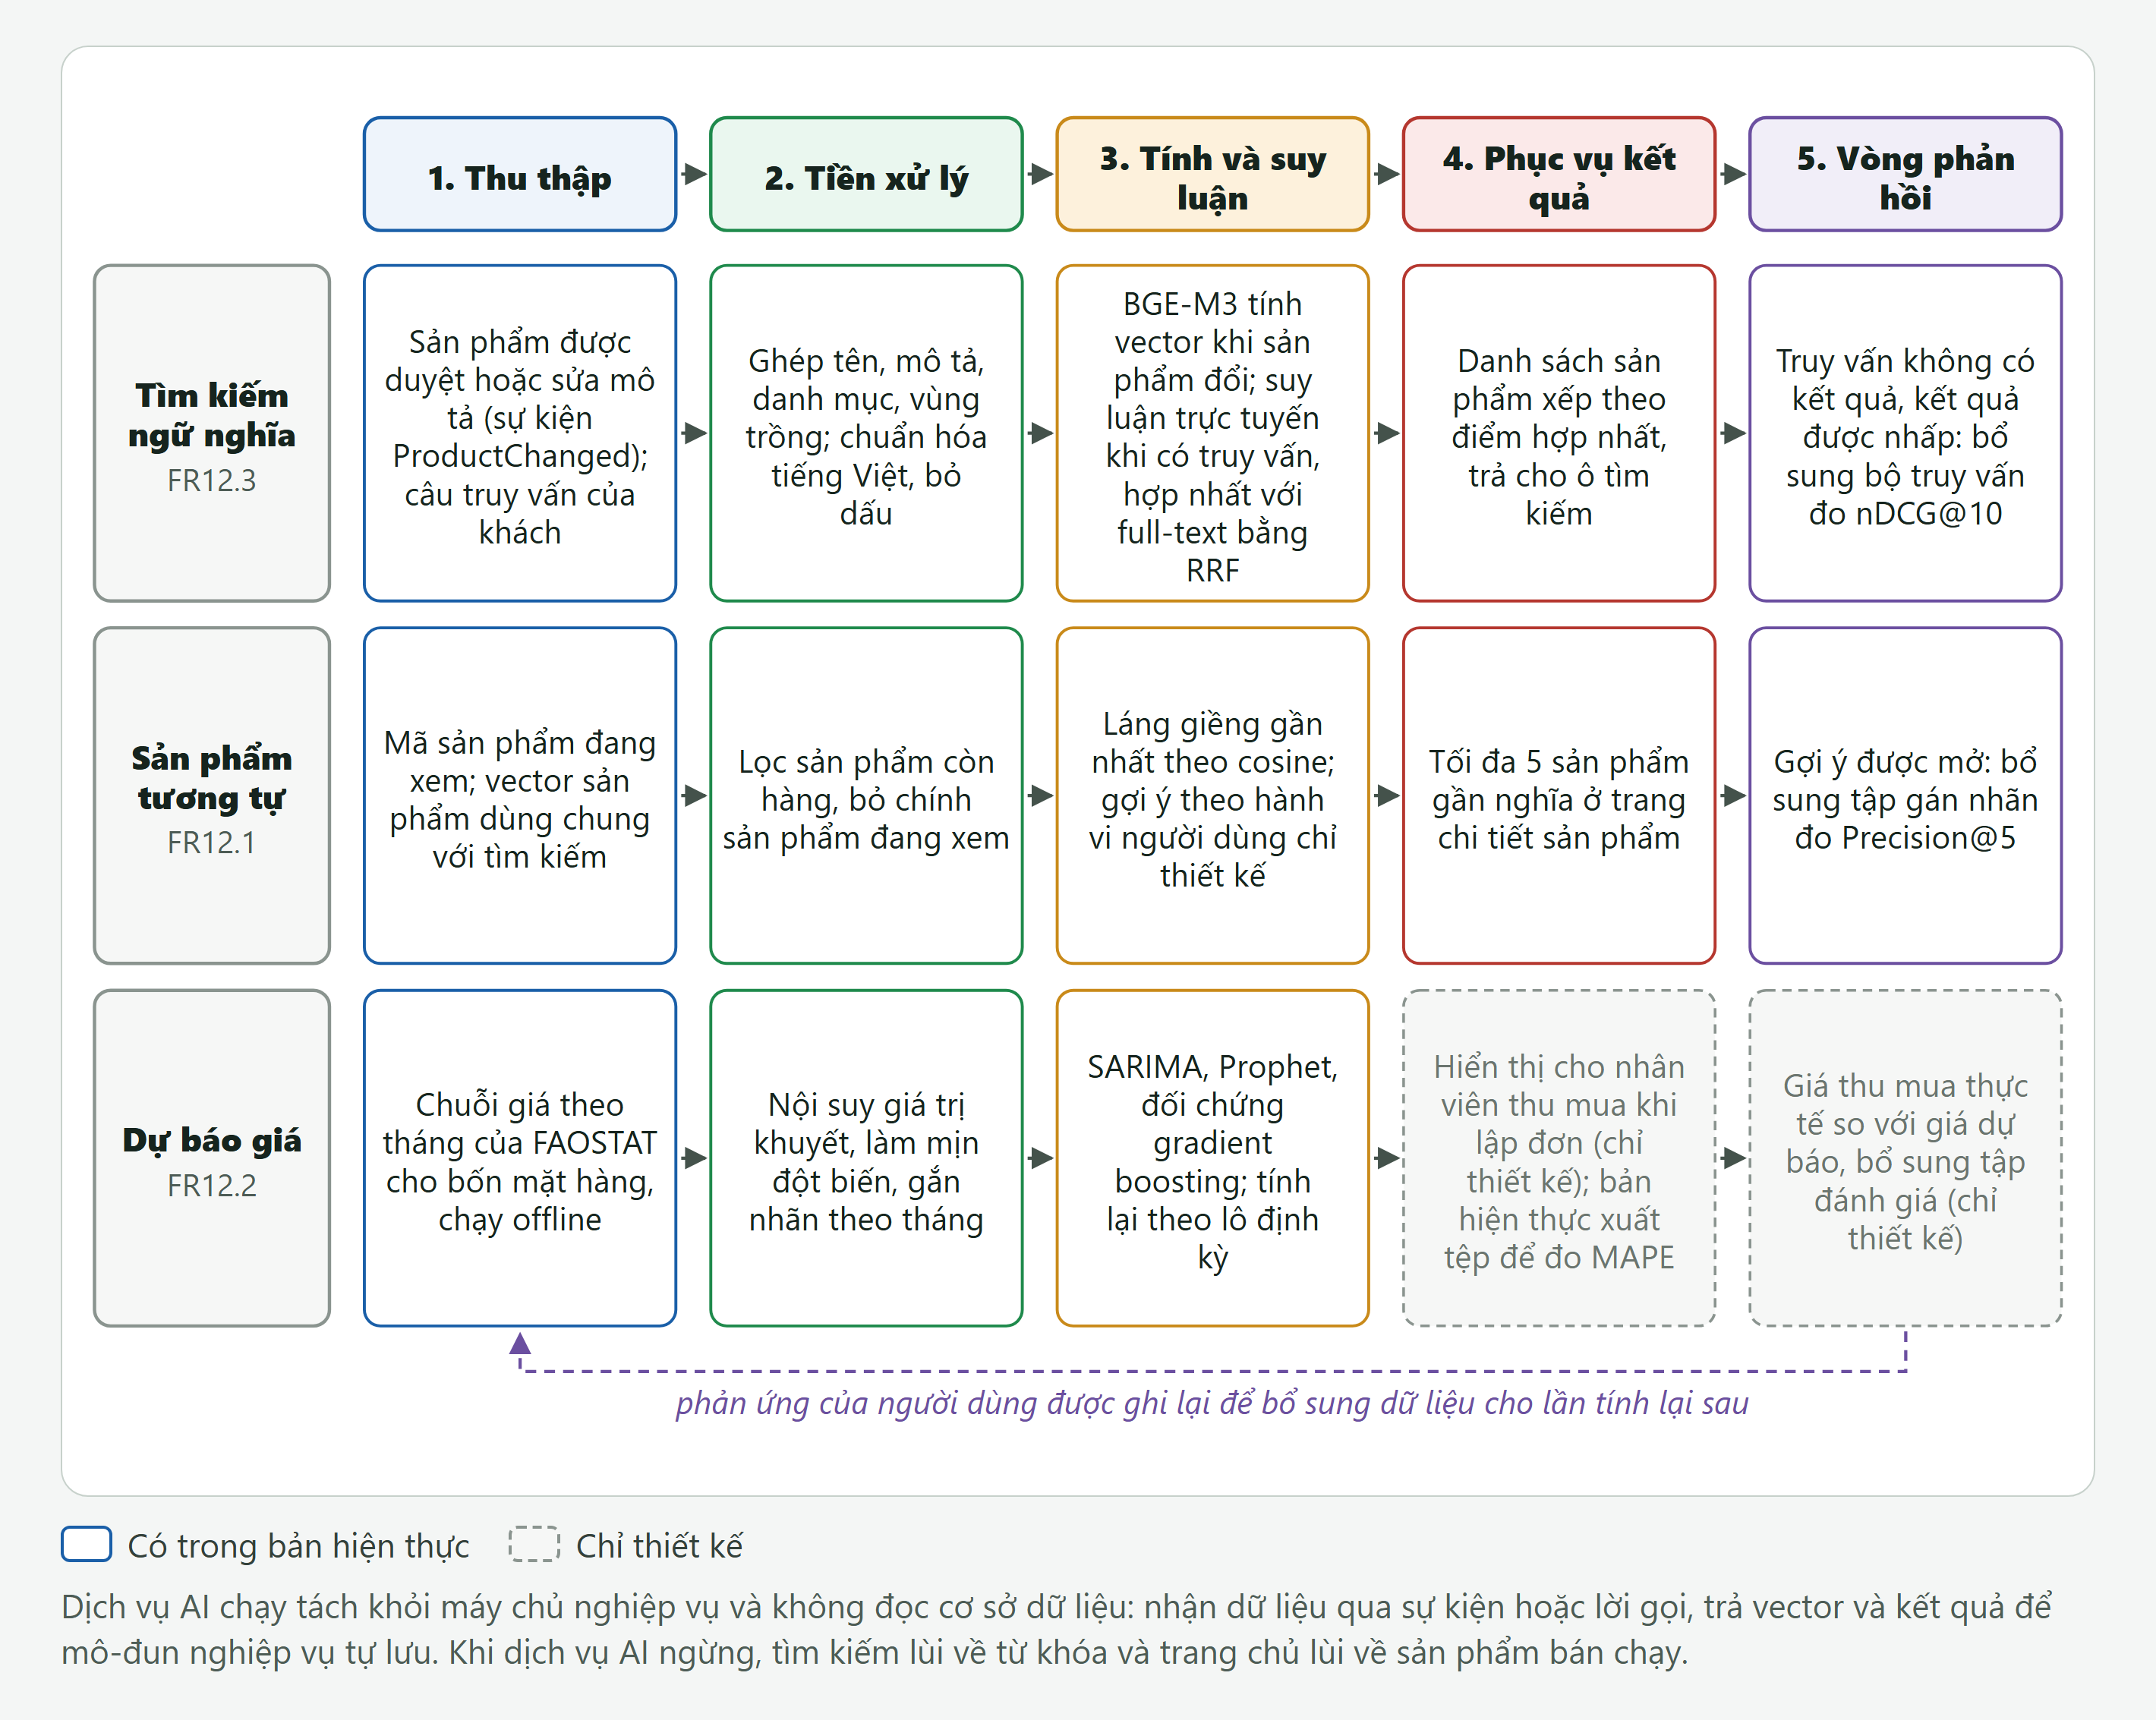
\includegraphics[width=\textwidth]{image/comparison/ai-luong-du-lieu.png}
\end{adjustbox}
\caption{Luồng dữ liệu năm bước của ba tính năng AI}
\label{fig:ai-luong}
\end{figure}

\begingroup
\tblsetup\tblzebra
\begin{longtable}{L{2.30cm} L{4.20cm} L{4.20cm} L{4.20cm}}
\caption{Ba tính năng AI của Farmery}
\label{tab:tinhnangAI} \\
\toprule
\rowcolor{tblheadbg}
& \textbf{Tìm kiếm ngữ nghĩa (FR12.3)} & \textbf{Sản phẩm tương tự (FR12.1)} & \textbf{Dự báo giá (FR12.2)} \\
\midrule
\endfirsthead
\toprule
\rowcolor{tblheadbg}
& \textbf{Tìm kiếm ngữ nghĩa (FR12.3)} & \textbf{Sản phẩm tương tự (FR12.1)} & \textbf{Dự báo giá (FR12.2)} \\
\midrule
\endhead
\bottomrule
\endfoot
\textbf{Ai dùng, ở đâu} & Khách vãng lai, khách lẻ; ô tìm kiếm của ứng dụng mua hàng & Khách vãng lai, khách lẻ; trang chi tiết sản phẩm & Nhân viên thu mua; màn hình lập đơn \emph{(chỉ thiết kế)}, bản hiện thực chưa có màn hình \\
\textbf{Vào $\rightarrow$ ra} & Câu truy vấn hoặc từ khóa (không dấu, sai chính tả) $\rightarrow$ sản phẩm xếp theo điểm hợp nhất & Mã sản phẩm đang xem $\rightarrow$ tối đa 5 sản phẩm gần nghĩa nhất đang bán & Loại nông sản, chuỗi giá theo tháng $\rightarrow$ giá dự báo kèm khoảng tin cậy, xuất tệp để đo MAPE \\
\textbf{Mô hình} & Full-text PostgreSQL (\texttt{unaccent}, trigram) cộng vector BGE-M3, hợp nhất bằng reciprocal rank fusion & Láng giềng gần nhất theo cosine trên vector BGE-M3, lọc còn hàng & Chuỗi thời gian có mùa vụ (SARIMA, Prophet), đối chứng gradient boosting \\
\textbf{Dữ liệu} & Tên, mô tả, danh mục, vùng trồng của sản phẩm đã duyệt; vector tính lại khi sản phẩm đổi & Vector dùng chung với tìm kiếm & Giá nhà sản xuất theo tháng của FAOSTAT cho mặt hàng có chuỗi đủ dài; chạy offline theo lô \\
\textbf{Chỉ số} & nDCG@10, Recall@10 so với tìm từ khóa trên tối thiểu 50 truy vấn gán nhãn tay; p95 dưới 1 giây & Precision@5 trên tập gán nhãn tay & MAPE trên tập kiểm tra tách theo thời gian \\
\textbf{Mức hiện thực} & Hiện thực; tìm nhà cung cấp cho khách sỉ \emph{chỉ thiết kế} & Hiện thực; cá nhân hóa theo hành vi \emph{chỉ thiết kế} & Offline, đo MAPE; hiển thị cho nhân viên thu mua \emph{chỉ thiết kế} \\
\end{longtable}
\endgroup

\noindent\textbf{Ngưỡng chất lượng mục tiêu.}\label{subsec:nguongAI} Vì cả ba mô-đun chưa có dữ liệu vận hành thật, ngưỡng được đặt ngay từ bước thiết kế để làm căn cứ đối chiếu ở Chương~\ref{chap:danhgia}: nDCG@10 và Recall@10 so với tìm từ khóa, Precision@5 trên tập gán nhãn tay, MAPE cho dự báo giá; mức tăng CTR chỉ dùng khi bật gợi ý cá nhân hóa \emph{(chỉ thiết kế)}. Bảng~\ref{tab:nguongAI} (Phụ lục~E) nêu từng ngưỡng kèm lý do chọn.

\subsection{Chính sách đối với xử lý của hệ thống và các bên thứ ba}
\label{subsec:chinhsachbenthuba}

\begin{itemize}
    \item \textbf{Cổng thanh toán:} mọi thanh toán và hoàn tiền qua cổng được cấp phép, hệ thống chỉ lưu mã giao dịch để đối soát, không lưu dữ liệu thẻ (NFR3.4); kết quả chỉ được ghi nhận khi webhook có chữ ký hợp lệ và gửi lại nhiều lần chỉ xử lý một lần. Kết nối thật và ký quỹ (FR7.3) \emph{chỉ thiết kế}; bản hiện thực dùng cổng giả lập sau cùng giao diện tích hợp.
    \item \textbf{Đơn vị vận chuyển chặng cuối (3PL):} tạo vận đơn qua REST và nhận trạng thái qua webhook \emph{(chỉ thiết kế)}; bản hiện thực để nhân viên vận hành chuyển bước. Thời gian chờ tối đa 5 giây và thử lại khi lỗi tạm thời (NFR7.1) áp cho mọi lời gọi qua lớp tích hợp, kể cả giả lập; lỗi của 3PL do Farmery xử lý với khách trước, đòi lại sau.
    \item \textbf{Hóa đơn điện tử và đăng nhập bên thứ ba:} hóa đơn giả lập qua cùng giao diện nhà cung cấp thật sẽ dùng, nên khi kết nối thật chỉ đổi lớp tích hợp (FR7.2, NFR8.3); đăng nhập Google, Facebook \emph{(chỉ thiết kế)} vẫn phải xác thực OTP cho thao tác nhạy cảm (FR1.1, FR1.2).
    \item \textbf{Xác minh chứng nhận và xử lý nội bộ:} xác minh làm thủ công, chuyển sang đối chiếu tự động khi có kết nối với cơ quan cấp; giới hạn tần suất (khóa 30 phút sau 5 lần sai), khóa tồn khi đặt hàng, lưu vết mọi thao tác quản trị (NFR3.5, NFR1.2).
\end{itemize}
